\documentclass{tudelft-report}
\usepackage{natbib}
% Start of 'ignore natbib' hack
\let\bibhang\relax
\let\citename\relax
\let\bibfont\relax
\let\Citeauthor\relax
\expandafter\let\csname ver@natbib.sty\endcsname\relax
\usepackage{changes}
\usepackage{subcaption}
\usepackage[export]{adjustbox}
\usepackage{float}
\restylefloat{table}
\usepackage[style=authoryear-ibid,backend=biber]{biblatex}
\usepackage{csquotes}
%%\addbibresource{report.bib}
\begin{document}
%% Use Roman numerals for the page numbers of the title pages and table of
%% contents.
\frontmatter

%% Uncomment following 19 lines for a cover with a picture on the lower half only
%\title[tudelft-white]{Title}
%\subtitle[tudelft-cyan]{Optional subtitle}
%\author[tudelft-white]{J.\ Random Author}
%\affiliation{Technische Universiteit Delft}
%\coverimage{cover.jpg}
%\titleoffsetx{10cm}
%\titleoffsety{10cm}
%\afiloffsetx{1cm}
%\afiloffsety{18cm}
%\covertext[tudelft-white]{
%    \textbf{Cover Text} \\
%    possibly \\
%    spanning 
%    multiple 
%    lines
%    \vfill
%    ISBN 000-00-0000-000-0
%}
%\makecover
%% Uncomment following 16 lines for a cover with a picture on the lower half only
\title[tudelft-white]{\fontsize{30}{5}\fontshape{sl}\selectfont Identifying movement patterns from large scale WiFi-based location data}
\subtitle[tudelft-white]{\fontsize{20}{1.2}\selectfont\hspace{5cm}    -A case study of TU Delft Campus}
\author[tudelft-white]{\fontsize{15}{10}\selectfont Balazs Dukai
\vskip 0.15cm Simon Griffioen
\vskip 0.15cm Matthijs Bon
\vskip 0.15cm Martijn Vermeer
\vskip 0.15cm Xander den Duijn
\vskip 0.15cm Yuxuan Kang}
\affiliation{Technische Universiteit Delft}
\coverimage{cover_article.jpg}

\setpagecolor{tudelft-cyan}
\makecover[split]

%% Include an optional title page.
%%\begin{titlepage}


\begin{center}

%% Insert the TU Delft logo at the bottom of the page.

%% Print the title in cyan.
{\makeatletter
\largetitlestyle\fontsize{64}{94}\selectfont\@title
%\largetitlestyle\color{tudelft-cyan}\Huge\@title
\makeatother}

%% Print the optional subtitle in black.
{\makeatletter
\ifx\@subtitle\undefined\else
    \bigskip
   {\tudsffamily\fontsize{22}{32}\selectfont\@subtitle}    
    %\titlefont\titleshape\LARGE\@subtitle
\fi
\makeatother}

\bigskip
\bigskip

by
%door

\bigskip
\bigskip

%% Print the name of the author.
{\makeatletter
%\largetitlefont\Large\bfseries\@author
\largetitlestyle\fontsize{26}{26}\selectfont\@author
\makeatother}

\bigskip
\bigskip

{\fontsize{15}{0.2}\selectfont Synthesis project of Geomatics
%ter verkrijging van de graad van Master of Science

at the Delft University of Technology,}
%aan de Technische Universiteit Delft,

\vfill

\begin{tabular}{lll}
    Project duration: & \multicolumn{2}{l}{April 16, 2016 -- June 17, 2016} \\
\end{tabular}
%% Only include the following lines if confidentiality is applicable.

\bigskip
\bigskip
\bigskip
\bigskip
%\\[1cm]
to be presented on Friday May 20, 2016.
\end{center}

\begin{tikzpicture}[remember picture, overlay]
    \node at (current page.south)[anchor=south,inner sep=0pt]{
        
\includegraphics{cover/logo_black}
    };
\end{tikzpicture}

\end{titlepage}



%%\chapter*{Preface}
During the fourth quarter of the first year of the MSc Programme Geomatics for the Built Environment at the TU Delft, the Geomatics Synthesis Project (GSP) takes place. This report is part of this framework and in this project, students will apply all their knowledge they have acquired during the courses while working in groups of five or six students. The students will gain experience throughout the entire process of project management, data processing, data analysis, application and presentation. \\\\
This year, the GSP focusses on Wi-Fi tracking data from the eduroam network of the TU Delft. The student will be divided into three groups, each researching one of three different topics:
\begin{itemize}
\item Identifying occupancy
\item Identifying movement patterns
\item Identifying activities
\end{itemize}
This project is dedicated to the second topic, identifying movement patterns. The project requires 3 main documents: \begin {enumerate*} [label=\itshape\arabic*\upshape),font={\color{red!0!black}\bfseries}] \item the baseline review; \item the mid term review, and \item the final review
\end{enumerate*}
This document embodies the final review and was created to provide the students, the supervisor(s) and other involved parties with an overview of the project. The document includes the problem description, development process, results, conclusions and recommendations for future work.
\\\\
\\\\
\\\\
\\\\
Delft, University of Technology\\

\begin{flushleft}
{\makeatletter\itshape
    \@author\\
    Delft, June 2016
\makeatother}
\end{flushleft}



%%\tableofcontents

%% Use Arabic numerals for the page numbers of the chapters.
\mainmatter
%%\setcounter{chapter}{-1}
\chapter{abstract}
This document is intended to be both an example of the TU Delft \LaTeX{} template for reports and theses, as well as a short introduction to its use. It is not intended to be a general introduction to \LaTeX{} itself,\footnote{We recommend \url{http://en.wikibooks.org/wiki/LaTeX} as a reference and a starting point for new users.} and we will assume the reader to be familiar with the basics of creating and compiling documents.

Instructions on how to use this template under Windows and Linux, and which \LaTeX{} packages are required, can be found in \texttt{README.txt}.


Since a report, and especially a thesis, might be a substantial document, it is convenient to break it up into smaller pieces. In this template we therefore give every chapter its own file. The chapters (and appendices) are gathered together in \texttt{report.tex}, which is the master file describing the overall structure of the document. \texttt{report.tex} starts with the line
\begin{quote}
    \texttt{\textbackslash documentclass\{tudelft-report\}}
\end{quote}
which loads the TU Delft report template. The template is based on the \LaTeX{} \texttt{book} document class and stored in \texttt{tudelft-report.cls}. The document class accepts several comma-separated options. The default language is English, but this can be changed to Dutch (\emph{e.g.}, for bachelor theses) by specifying the \texttt{dutch} option:
\begin{quote}
    \texttt{\textbackslash documentclass[dutch]\{tudelft-report\}}
\end{quote}
Furthermore, hyperlinks are shown in blue, which is convenient when reader the report on a computer, but can be expensive when printing. They can be turned black with the \texttt{print} option. This will also turn the headers black instead of cyan.

If the document becomes large, it is easy to miss warnings about the layout in the \LaTeX{} output. In order to locate problem areas, add the \texttt{draft} option to the \texttt{\textbackslash documentclass} line. This will display a vertical bar in the margins next to the paragraphs that require attention. Finally, the \texttt{nativefonts} option can be used to override the automatic font selection (see below).

This template has the option to automatically generate a cover page with the \texttt{\textbackslash makecover} command. See the next section for a detailed description.

The contents of the report are included between the \texttt{\textbackslash begin\{document\}} and \texttt{\textbackslash end\{document\}} commands, and split into three parts by
\begin{enumerate}
\item\texttt{\textbackslash frontmatter}, which uses Roman numerals for the page numbers and is used for the title page and the table of contents;
\item\texttt{\textbackslash mainmatter}, which uses Arabic numerals for the page numbers and is the style for the chapters;
\item\texttt{\textbackslash appendix}, which uses letters for the chapter numbers, starting with `A'.
\end{enumerate}
The title page is defined in a separate file, \emph{e.g.}, \texttt{title.tex}, and included verbatim with \texttt{\textbackslash input\{title\}}.\footnote{Note that it is not necessary to specify the file extension.} Additionally, it is possible to include a preface, containing, for example, the acknowledgements. An example can be found in \texttt{preface.tex}. The table of contents is generated automatically with the \texttt{\textbackslash tableofcontents} command. Chapters are included after \texttt{\textbackslash mainmatter} and appendices after \texttt{\textbackslash appendix}. For example, \texttt{\textbackslash input\{chapter-1\}} includes \texttt{chapter-1.tex}, which contains this introduction.

The bibliography, finally, is generated automatically with
\begin{quote}
    \texttt{\textbackslash bibliography\{report\}}
\end{quote}
from \texttt{report.bib}. The bibliography style is specified in \texttt{tudelft-report.bst}, which is a modified version of \texttt{apsrev4-1.bst} (from REVTeX) designed to also display the titles of referenced articles. The template will automatically generate clickable hyperlinks if a URL or DOI (digital object identifier) is present for the reference. As an example, we cite the paper by Nobel laureate Andrei Geim and his pet hamster \citep{Geim2001}. Although it is possible to manage the bibliography by hand, we recommend using EndNote (available from Blackboard) or JabRef (available from \url{http://jabref.sourceforge.net/}).


This template will automatically generate a cover page if you issue the \texttt{\textbackslash makecover} command. There are two formats for the cover page: one with a page-filling (`bleeding')
illustration, with the title(s) and author(s) in large ultrathin typeface, and the other where the illustration fills the lower half of the A4, whereas title(s), author(s) and additional
text are set in the standard sans-serif font on a plain background with a color chosen by the user. The last option is selected by the optional key \texttt{split}: \texttt{\textbackslash makecover[split]} yields
a page with the illustration on the lower half. All illustrations are bleeding, in accordance with the TU Delft style.

Before generating the cover, you need to provide the information to put on it. This can be done with the following commands:
\begin{itemize}
\item\texttt{\textbackslash title[Optional Color]\{Title\}} \\
    This command is used to provide the title of the document. The title
    title is also printed on the spine. If you use a title page (see below), this information will be used there as well.
    As the title, subtitle and author name are printed directly over the cover photo, it will often be necessary to adjust the print color in order to have
    sufficient contrast between the text and the background. The optional color argument is used for this.
\item\texttt{\textbackslash title[Optional Color]\{Subtitle\}} \\
    This command is used to provide a subtitle for the document. If you use a title page (see below), this information will be used there as well.
    It possible to adjust the print color in order to have
    sufficient contrast between the text and the background -- the optional color argument is used for this.
\item\texttt{\textbackslash author\{J.\ Random Author\}} \\
    This command specifies the author. The default color is \texttt{tudelft-white}, but this may be adjusted in the same way as the titles.
\item\texttt{\textbackslash affiliation\{Technische Universiteit Delft\}} \\
    The affiliation is the text printed vertically on the front cover. It can be the affiliation, such as the university or department name, or be used for the document type (\emph{e.g.}, Master's thesis). The default color is again \texttt{tudelft-white}, adjustable through the \texttt{color} option.
\item\texttt{\textbackslash coverimage\{cover.jpg\}} \\
    With this command you can specify the filename of the cover image. The image is stretched to fill the full width of the front cover (including the spine if a back cover is present).
\item\texttt{\textbackslash covertext\{Cover Text\}} \\
    If a back cover is present, the cover text is printed on the back. Internally, this text box is created using the \LaTeX{} \texttt{minipage} environment, so it supports line breaks.
\item\texttt{\textbackslash titleoffsetx\{OffsetX\},\textbackslash titleoffsety\{OffsetY\}}
    If the cover page contains a page-filling picture (i.e., \texttt{split} is not specified with the \texttt{makecover} command, the best position of the title depends a lot on the picture chosen for it. The lower left corner of the minipage containing title, subtitle and author is 
    specified by these two commands. The offsets are measured from the top left corner of the page. 
\item\texttt{\textbackslash afiloffsetx\{AfilX\}, \textbackslash afiloffsety\{AfilY\}}
    specifies the lower left corner of the text containing the affiliation, measured from the top left corner of the page. 
\end{itemize}

In addition to \texttt{[split]}, the \texttt{\textbackslash makecover} command accepts several additional options for customizing the layout of the cover. 
The most important of these is \texttt{back}. Supplying this option will generate a back cover as well as a front, including the spine. Since this requires a page size slightly larger than twice A4 (to make room for the spine), and \LaTeX{} does not support different page sizes within the same document, it is wise to create a separate file for the cover. \texttt{cover.tex} contains an example. The recommended page size for the full cover can be set with
\begin{quote}
    \textbackslash geometry\{papersize=\{1226bp,851bp\}\}
\end{quote}
after the document class and before \texttt{\textbackslash begin\{document\}}.

The other options \texttt{\textbackslash makecover} accepts are
\begin{itemize}
\item\texttt{nospine} \\
    If a back cover is generated, the title will also be printed in a black box on the spine. However, for smaller documents the spine might not be wide enough. Specifying this option disables printing the title on the spine.
\item\texttt{frontbottom} \\
    By default the black box on the front is situated above the blue box. Specifying this option will place the black box below the blue one.
\item\texttt{spinewidth} \\
    If a back cover is present, this option can be used to set the width of the spine. The default is \texttt{spinewidth=1cm}.
\item\texttt{frontboxwidth}, \texttt{frontboxheight}, \texttt{backboxwidth}, \texttt{backboxheight} \\
    As their names suggest, these options are used to set the width and height of the front (black) and back (blue) boxes. The default widths and heights are \texttt{4.375in} and \texttt{2.1875in}, respectively.
\item\texttt{x}, \texttt{y} \\
    The blue and black boxes touch each other in a corner. The location of this corner can be set with these options. It is defined with respect to the top left corner of the front cover. The default values are \texttt{x=0.8125in} and \texttt{y=3in}.
\item\texttt{margin} \\
    This option sets the margin between the borders of the boxes and their text. The default value is \texttt{12pt}.
\end{itemize}

For a thesis it is desirable to have a title page within the document, containing information like the thesis committee members. To give you greater flexibility over the layout of this page, it is not generated by a command like \texttt{\textbackslash makecover}, but instead described in the file \texttt{title.tex}. Modify this file according to your needs. The example text is in English, but Dutch translations are provided in the comments. Note that for a thesis, the title page is subject to requirements which differ by faculty. Make sure to check these requirements before printing.

Each chapter has its own file. For example, the \LaTeX{} source of this chapter can be found in \texttt{chapter-1.tex}. A chapter starts with the command
\begin{quote}
    \texttt{\textbackslash chapter\{Chapter title\}}
\end{quote}
This starts a new page, prints the chapter number and title and adds a link in the table of contents. If the title is very long, it may be desirable to use a shorter version in the page headers and the table of contents. This can be achieved by specifying the short title in brackets:
\begin{quote}
    \texttt{\textbackslash chapter[Short title]\{Very long title with many words which could not possibly fit on one line\}}
\end{quote}
Unnumbered chapters, such as the preface, can be created with \texttt{\textbackslash chapter*\{Chapter title\}}. Such a chapter will not show up in the table of contents or in the page header. To create a table of contents entry anyway, add
\begin{quote}
    \texttt{\textbackslash addcontentsline\{toc\}\{chapter\}\{Chapter title\}}
\end{quote}
after the \texttt{\textbackslash chapter} command. To print the chapter title in the page header, add
\begin{quote}
    \texttt{\textbackslash setheader\{Chapter title\}}
\end{quote}

Chapters are subdivided into sections, subsections, subsubsections, and, optionally, paragraphs and subparagraphs. All can have a title, but only sections and subsections are numbered. As with chapters, the numbering can be turned off by using \texttt{\textbackslash section*\{\ldots\}} instead of \texttt{\textbackslash section\{\ldots\}}, and similarly for the subsection.

\paragraph{\textbackslash paragraph\{\ldots\}}
Lorem ipsum dolor sit amet, consectetur adipisicing elit, sed do eiusmod tempor incididunt ut labore et dolore magna aliqua. Ut enim ad minim veniam, quis nostrud exercitation ullamco laboris nisi ut aliquip ex ea commodo consequat. Duis aute irure dolor in reprehenderit in voluptate velit esse cillum dolore eu fugiat nulla pariatur. Excepteur sint occaecat cupidatat non proident, sunt in culpa qui officia deserunt mollit anim id est laborum.


The fonts used by this template depend on which version of \LaTeX{} you use. Regular \LaTeX, \emph{i.e.}, if you compile your document with with \texttt{latex}, \texttt{pslatex} or \texttt{pdflatex}, will use Utopia for text, Fourier for math and Latin Modern for sans-serif and monospaced text. 
However, if you want to adhere to the TU Delft house style, you will need to use \XeLaTeX, as it supports TrueType and OpenType fonts. Compiling with \texttt{xelatex} will use Arial for most titles and text, Courier New for monospace and Cambria for math. If you want to haf a sans-serif font for the
main text, while using \texttt{latex}, \texttt{pslatex} or \texttt{pdflatex}, you can use the option \texttt{noroman} in the report style: \texttt{\textbackslash usepackage[\ldots,noroman]{tudelft-report}}. For document and part titles,  TU Delft Ultra Light is used. For quotes, columns and text in boxes, you use Georgia. If you want to use \XeLaTeX, but do not want to use the TU Delft house style fonts, you can add the \texttt{nativefonts} option to the document class. This will still use  TU Delft Utra Light and Arial on the cover, but not for the body of the document. If you need to use these fonts for certain sections in the main text, they are available via \texttt{\textbackslash tudrmfamily} (Georgia) and \texttt{\textbackslash tudtitlefamily} (TU Delft Utra Light).

\begin{quote}
  You have to learn the rules of the game. And then you have to play better than anyone else.\\
  \emph{Albert Einstein}
\end{quote}

The corporate colors of the TU Delft are cyan, black and white, available via \texttt{\textbackslash color\{{\color{tudelft-cyan}tudelft-cyan}\}}, \texttt{\textbackslash color\{{\color{tudelft-black}tudelft-black}\}} (which differs slightly from the default \texttt{\textbackslash color\{black\}}) and \texttt{\textbackslash color\{tudelft-white\}}, respectively. Apart from these three, the house style defines the basic colors \texttt{\color{tudelft-sea-green}tudelft-sea-green}, \texttt{\color{tudelft-green}tudelft-green}, \texttt{\color{tudelft-dark-blue}tudelft-dark-blue}, \texttt{\color{tudelft-purple}tudelft-purple}, \texttt{\color{tudelft-turquoise}tudelft-turquoise} and \texttt{\color{tudelft-sky-blue}tudelft-sky-blue}, as well as the accent colors \texttt{\color{tudelft-lavendel}tudelft-lavendel}, \texttt{\color{tudelft-orange}tudelft-orange}, \texttt{\color{tudelft-warm-purple}tudelft-warm-purple}, \texttt{\color{tudelft-fuchsia}tudelft-fuchsia}, \texttt{\color{tudelft-bright-green}tudelft-bright-green} and \texttt{\color{tudelft-yellow}tudelft-yellow}.


% Beginning of a chapter
% Use labels for referencing
\chapter{Movement patterns}\label{movementpatterns} 
\section{Introduction}\label{intro}
% this is a comment
% normal text
Lorem ipsum dolor sit amet, consectetur adipiscing elit. Cras placerat dolor at nibh dapibus condimentum. Aenean hendrerit libero eget leo consequat varius. Nullam in mollis purus. Vestibulum id interdum magna. Aliquam a ex dolor. Pellentesque nec dolor lorem. Nunc condimentum ac diam vitae rutrum. Quisque vulputate lobortis varius. In interdum dolor justo, eget laoreet leo pretium sit amet. \\ % newline
Lorem ipsum dolor sit amet, consectetur adipiscing elit. In tincidunt cursus massa ullamcorper placerat. Suspendisse eu justo lorem. Aliquam erat volutpat. Etiam neque enim, gravida id luctus nec, semper id felis. Sed dolor orci, consectetur id consectetur nec, rutrum vitae quam. Duis vel lobortis nisi. Suspendisse vel nibh ut est aliquam sollicitudin id quis odio. Nunc accumsan at massa ac interdum. Donec sit amet sem eu nibh imperdiet accumsan a eu risus. Nam euismod elit nec elit blandit, sed condimentum augue dapibus. Nulla fermentum velit sit amet tincidunt mattis. \\
Vivamus ut nulla id nisl imperdiet vulputate. Duis ornare egestas neque, porttitor fringilla dui iaculis imperdiet. Nulla facilisi. Sed odio diam, tempor eu metus a, laoreet feugiat tellus.\\
Begin numbered list
\begin{enumerate}
\item number 1
\item number 2
\item number 3
\item number 4
\end{enumerate}
Begin bullet list
\begin{itemize}
\item this is a bullet
\item this as well
\end{itemize}


\section{Include graphics}
To include graphics in the document, use the following template:

\begin{figure}[H]
\centering
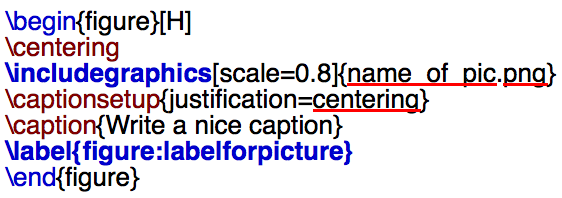
\includegraphics[scale=0.8]{name_of_pic.png}
\captionsetup{justification=centering}
\caption{Write a nice caption}
\label{figure:labelforpicture}
\end{figure}

If you want to refer to a picture (or section/chapter/whatever) in the text, this can be done using the 'autoref' function. \autoref{figure:labelforpicture} shows how to include graphics in a document. This also works for sections: \autoref{movementpatterns}.

\section{Tables}
Use \url{http://www.tablesgenerator.com} for creating nice looking tables. Use the 'booktabs' style!!!
\begin{table}[H]
\centering
\caption{My caption}
\label{my-label}
<<<<<<< HEAD
\begin{tabular}{lll}[H]
\hline
this & is      & a      \\ \hline
=======
\begin{tabular}{@{}lll@{}}
\toprule
this & is      & a      \\ \midrule
>>>>>>> 3dc9814e185ffebcba50bc64c0886fdaf49dc3d0
nice & looking & table  \\
am   & i       & right? \\ \bottomrule
\end{tabular}
\end{table}
Unfortunately, LaTeX always places tables at the top or bottom of a page, so it will mostly mess up the layout! Use proper referencing in the text to make sure tables are read as they should! \autoref{my-label}.

\section{Referencing}
It would be nice if everyone could go over the parts they have written in the mid-term review and find everything they have referenced. You can easily import biblatex styled references from google scholar. If you search in google scholar for a title, there is usually a link below the result, 'cite'. Then you can select 'bibtex' as an option to download a file. The text inside this file can be copied into the 'report.bib' file. If you want to cite an author, that can be done using the 'cite' option. i.e. this author was used in the mid term review:
Let's cite! The Einstein's journal paper \cite{mautz2012indoor} and the Dirac's 
book \cite{meneses2012large} are physics related items. 

\section{bold and italics}
\textbf{this text will be bold!}
\textit{this text will be in italics}





\chapter{Top level requirements}
To keep track of the progress of the project, it is necessary to monitor to which degree the project is meeting the top level requirements and if the project is still on schedule with these requirements. In the baseline review the requirements are specified using the MoSCoW rules and killer requirements. In this chapter these previous requirements will be discussed and possible changes will be explained.

The goals that \textit{must} be achieved is on the level of detail of the campus. It’s detailed specification as stated in the baseline review is shown below. 

\textbf{MUST} campus level
Main goal: 
\begin{enumerate}
\item Identify which entrances are used to enter and exit a building;
\item Identify movement patterns and connectivity between building entrances by sequential pattern mining.
\end{enumerate}
Relate entrances (place) of buildings to the corresponding APs (location).
Find the stay places of each individual in order of the scan time.
Find individual trajectories by taking a time interval from a sequence of stay places.
Find the movement patterns, by deriving a sequence of common places shared by all trajectories.
Visualize the movement patterns between buildings in static maps.
A \textit{killer requirement} for this level is:
Identification of APs relating to an entrance of a building

Currently the project is progressed so far that it is possible to identify building patterns between buildings. The stay places of individuals and their trajectories have been found and this has been visualized in both static and dynamic maps and bar charts. But, until now there is no accurate map with the location of all access points of the campus. There is such a map for the faculty of architecture, but it is only one building and not very clear. Until this map of the whole campus becomes available, identifying entrances will be hard to do. \autoref{entrance} will go into greater detail about the progress that has been made so far with entrances. 

The goals that \textit {should} be achieved, focus on the building level, where buildings are divided into regions, but since there is currently no map with the locations of the access points, this level of detail is not yet reached. However, the way that the code is setup allows for easy transformation to higher levels of detail when such a map becomes available. How this code exactly works is explained in \autoref{datadescr} and \autoref{movement between buildings}. 

\chapter{Progress}
\setcounter{secnumdepth}{4}
\setcounter{tocdepth}{4}
This document is intended to be both an example of the TU Delft \LaTeX{} template for reports and theses, as well as a short introduction to its use. It is not intended to be a general introduction to \LaTeX{} itself

Instructions on how to use this template under Windows and Linux, and which \LaTeX{} packages are required, can be found in \texttt{README.txt}.

\section{Movement between buildings}
\subsection{Bar chart}
\subsection{Maps}
In order to get an overview about how people move on the campus and further more,  find out movement patterns, a map visualization is essential. Map visualization consists of three parts: 
\begin{enumerate}
\item base map: open street map is used as base map. There are many labels on open street map, providing more context of the environment, so it is more clear and readable compared to other base maps like satellite images.
\item building markers: building markers show the locations of the buildings. Google maps marker style is used since it is commonly used in many map application. Because the shape of the building is not useful in analyzing movement patterns between buildings, each building is regarded as a point instead of a polygon, thus a node in the network, 
\item lines: lines are the most essential part in map visualization, they represent movements between buildings.
\end{enumerate}

In the first stage of map visualization, only base map and lines are taken into consideration, building markers are not shown on the map. The line width represents the amount of movement and movements are aggregated daily regardless of the timestamp of each movement during a day. This map visualization gives an overview of the movements over a day and between which buildings there are the most movements. The following maps show the difference of the amount of movement between April 11th (weekday) and April 17th (weekend).
\graphicspath{ {pics/} }
\begin{figure}[H]
\minipage{0.2\textwidth}
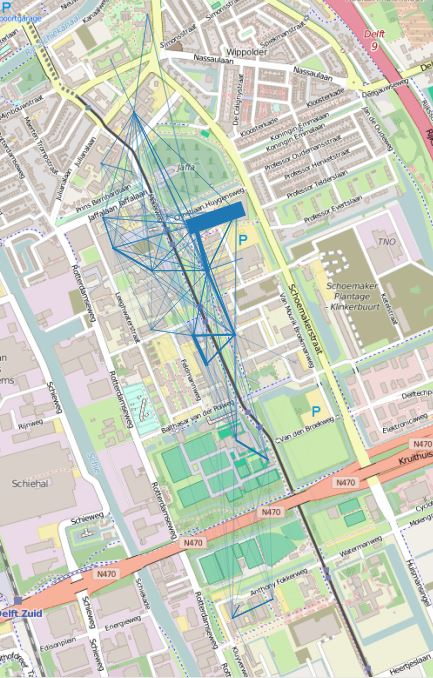
\includegraphics[scale=0.7,left]{pic1}
\captionsetup{justification=centering}
\caption{Movements of April 11th (week day)}
\endminipage\hfill
\minipage{0.2\textwidth}
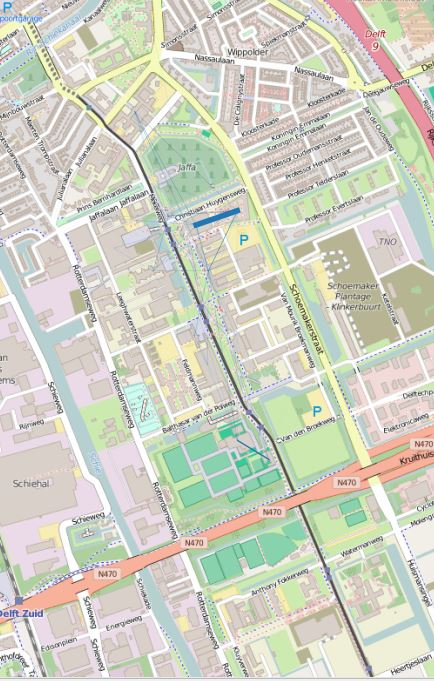
\includegraphics[scale=0.7,right]{pic2}
\captionsetup{justification=centering}
\caption{Movements of April 17th (weekend)}
\endminipage\hfill

\end{figure}
It's clear that between Aula and library, there are the most movements and the amount of movements is totally different on weekday and on weekend.

Regarding the movements are dynamic and time is also highly related to movements, a dynamic map visualization is created to display individual movement over a day with temporal information. The following screenshots of the gif file show how the movements look like at a certain time of a day:

\begin{figure}[H]
\minipage{0.2\textwidth}
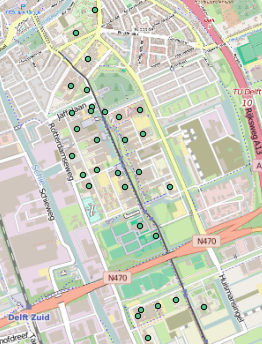
\includegraphics[scale=0.6,left]{frame009}
\captionsetup{justification=centering}
\caption{Movements of April 11th, 7:00 am}
\endminipage\hfill
\minipage{0.2\textwidth}
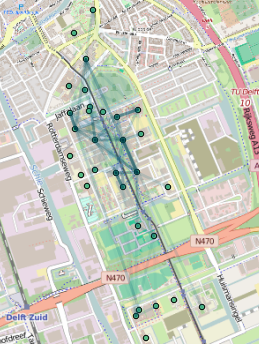
\includegraphics[scale=0.6,center]{frame021}
\captionsetup{justification=centering}
\caption{Movements of April 11th, 9:00 am}
\endminipage\hfill
\minipage{0.2\textwidth}
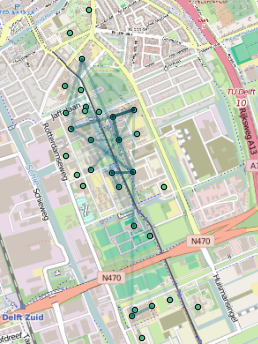
\includegraphics[scale=0.6,right]{frame033}
\captionsetup{justification=centering}
\caption{Movements of April 11th 11:00 am}
\endminipage\hfill
\end{figure}

\begin{figure}[H]
\minipage{0.2\textwidth}
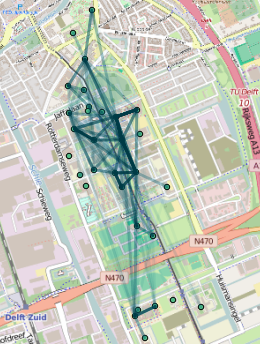
\includegraphics[scale=0.6,left]{frame045}
\captionsetup{justification=centering}
\caption{Movements of April 11th, 13:00 pm}
\endminipage\hfill
\minipage{0.2\textwidth}
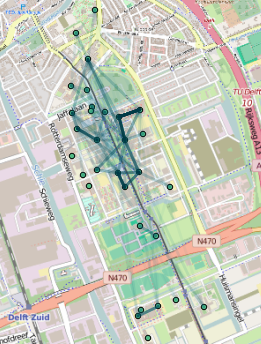
\includegraphics[scale=0.6,center]{frame057}
\captionsetup{justification=centering}
\caption{Movements of April 11th, 15:00 pm}
\endminipage\hfill
\minipage{0.2\textwidth}
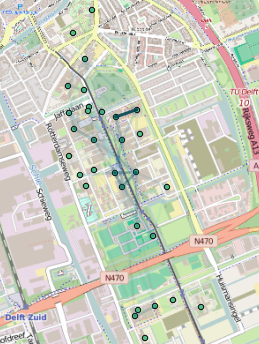
\includegraphics[scale=0.6,right]{frame066}
\captionsetup{justification=centering}
\caption{Movements of April 11th 16:30 pm}
\endminipage\hfill
\end{figure}

\begin{figure}[H]
\minipage[height=2]{0.2\textwidth}
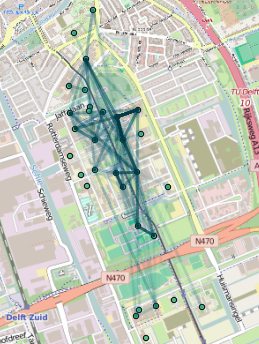
\includegraphics[scale=0.6,left]{frame075}
\captionsetup{justification=centering}
\caption{Movements of April 11th, 18:00 pm}
\endminipage\hfill
\minipage[height=2]{0.2\textwidth}
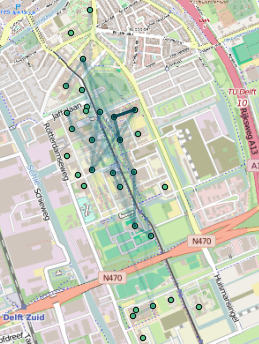
\includegraphics[scale=0.6,center]{frame087}
\captionsetup{justification=centering}
\caption{Movements of April 11th, 20:00 pm}
\endminipage\hfill
\minipage[height=2]{0.2\textwidth}
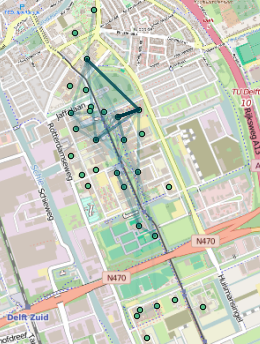
\includegraphics[scale=0.6,right]{frame099}
\captionsetup{justification=centering}
\caption{Movements of April 11th 22:00 pm}
\endminipage\hfill
\end{figure}

In these pictures, the more movements there are, the less transparent the lines are. So generally speaking, from 7:00 am to 20:00 pm, there are two peaks at 13:00 pm and 18:00 pm. Hence, it is possible to get some insights about movement patterns from the animation. However, the dynamic map visualization doesn't provide detailed information to dig into but only an overview. So in order to mine on movement patterns, it is necessary to create maps containing more information, including time, direction and so forth. 

Because the amount of data is big, it is more convenient to generate maps automatically so that it will fasten the progress of finding movement patterns. According to the three components of map, there is some information needed to be collected before visualizing movement on map. The locations of buildings are collected manually on Google earth based the campus map. These locations are exported as KML file and imported into QGIS. After adding geometry columns x and y, the csv file is created and imported into database. By using $ST\_MakePoint$ function, a geometry column is created in database. In summary, the building locations are stored as the structure described in following table:

\begin{table}[H]
\centering
\begin{tabular}{|c|c|c|c|c|}
\hline 
id & name & geometry & x & y \\
\hline
0 & world & & & \\
\hline
3 & science\_ center & 010100000042A7.. & 4.36939919846287 & 52.0072322181367 \\
\hline
5 & tnw\_ bio & 010100000043AE.. & 4.37120211221402 & 52.0086132164098 \\
\hline
8 & bk\_ city & 010100000077E3.. & 4.37053698152436 & 52.0056562098059 \\
\hline
12 & tnw\_ dct & 01010000007CA.. & 4.36891378927259 & 52.0040834950037\\
\hline
.. & ... & ....& .... &....\\
\hline	
\end{tabular}
\captionsetup{justification=centering}
\caption{Building data structure}
\label{table:1}
\end{table}

There is a special 'building' called $world$ in the database. It is not an actual location, it is a virtual location which is used if someone is not scanned on the campus in a period of time. After storing the locations of buildings in the database, these locations will be extracted automatically from database to generate maps. There are two properties of lines used to deliver information:
\begin{enumerate}
\item width: line width is used to represent the amount of movements, but the amount is aggregated for both directions.
\item color: color is gradient from red to green. Red line means the movement is not symmetric that much more people move in one direction than the other, while green line means the movement is symmetric.
\end{enumerate}

\section{Sequences}

This template will automatically generate a cover page if you issue the \texttt{\textbackslash makecover} command. There are two formats for the cover page: one with a page-filling (`bleeding')
illustration, with the title(s) and author(s) in large ultrathin typeface, and the other where the illustration fills the lower half of the A4, whereas title(s), author(s) and additional
text are set in the standard sans-serif font on a plain background with a color chosen by the user. The last option is selected by the optional key \texttt{split}: \texttt{\textbackslash makecover[split]} yields
a page with the illustration on the lower half. All illustrations are bleeding, in accordance with the TU Delft style.

Before generating the cover, you need to provide the information to put on it. This can be done with the following commands:
\begin{itemize}
\item\texttt{\textbackslash title[Optional Color]\{Title\}} \\
    This command is used to provide the title of the document. The title
    title is also printed on the spine. If you use a title page (see below), this information will be used there as well.
    As the title, subtitle and author name are printed directly over the cover photo, it will often be necessary to adjust the print color in order to have
    sufficient contrast between the text and the background. The optional color argument is used for this.
\item\texttt{\textbackslash title[Optional Color]\{Subtitle\}} \\
    This command is used to provide a subtitle for the document. If you use a title page (see below), this information will be used there as well.
    It possible to adjust the print color in order to have
    sufficient contrast between the text and the background -- the optional color argument is used for this.
\item\texttt{\textbackslash author\{J.\ Random Author\}} \\
    This command specifies the author. The default color is \texttt{tudelft-white}, but this may be adjusted in the same way as the titles.
\item\texttt{\textbackslash affiliation\{Technische Universiteit Delft\}} \\
    The affiliation is the text printed vertically on the front cover. It can be the affiliation, such as the university or department name, or be used for the document type (\emph{e.g.}, Master's thesis). The default color is again \texttt{tudelft-white}, adjustable through the \texttt{color} option.
\item\texttt{\textbackslash coverimage\{cover.jpg\}} \\
    With this command you can specify the filename of the cover image. The image is stretched to fill the full width of the front cover (including the spine if a back cover is present).
\item\texttt{\textbackslash covertext\{Cover Text\}} \\
    If a back cover is present, the cover text is printed on the back. Internally, this text box is created using the \LaTeX{} \texttt{minipage} environment, so it supports line breaks.
\item\texttt{\textbackslash titleoffsetx\{OffsetX\},\textbackslash titleoffsety\{OffsetY\}}
    If the cover page contains a page-filling picture (i.e., \texttt{split} is not specified with the \texttt{makecover} command, the best position of the title depends a lot on the picture chosen for it. The lower left corner of the minipage containing title, subtitle and author is 
    specified by these two commands. The offsets are measured from the top left corner of the page. 
\item\texttt{\textbackslash afiloffsetx\{AfilX\}, \textbackslash afiloffsety\{AfilY\}}
    specifies the lower left corner of the text containing the affiliation, measured from the top left corner of the page. 
\end{itemize}

In addition to \texttt{[split]}, the \texttt{\textbackslash makecover} command accepts several additional options for customizing the layout of the cover. 
The most important of these is \texttt{back}. Supplying this option will generate a back cover as well as a front, including the spine. Since this requires a page size slightly larger than twice A4 (to make room for the spine), and \LaTeX{} does not support different page sizes within the same document, it is wise to create a separate file for the cover. \texttt{cover.tex} contains an example. The recommended page size for the full cover can be set with
\begin{quote}
    \textbackslash geometry\{papersize=\{1226bp,851bp\}\}
\end{quote}
after the document class and before \texttt{\textbackslash begin\{document\}}.

The other options \texttt{\textbackslash makecover} accepts are
\begin{itemize}
\item\texttt{nospine} \\
    If a back cover is generated, the title will also be printed in a black box on the spine. However, for smaller documents the spine might not be wide enough. Specifying this option disables printing the title on the spine.
\item\texttt{frontbottom} \\
    By default the black box on the front is situated above the blue box. Specifying this option will place the black box below the blue one.
\item\texttt{spinewidth} \\
    If a back cover is present, this option can be used to set the width of the spine. The default is \texttt{spinewidth=1cm}.
\item\texttt{frontboxwidth}, \texttt{frontboxheight}, \texttt{backboxwidth}, \texttt{backboxheight} \\
    As their names suggest, these options are used to set the width and height of the front (black) and back (blue) boxes. The default widths and heights are \texttt{4.375in} and \texttt{2.1875in}, respectively.
\item\texttt{x}, \texttt{y} \\
    The blue and black boxes touch each other in a corner. The location of this corner can be set with these options. It is defined with respect to the top left corner of the front cover. The default values are \texttt{x=0.8125in} and \texttt{y=3in}.
\item\texttt{margin} \\
    This option sets the margin between the borders of the boxes and their text. The default value is \texttt{12pt}.
\end{itemize}

For a thesis it is desirable to have a title page within the document, containing information like the thesis committee members. To give you greater flexibility over the layout of this page, it is not generated by a command like \texttt{\textbackslash makecover}, but instead described in the file \texttt{title.tex}. Modify this file according to your needs. The example text is in English, but Dutch translations are provided in the comments. Note that for a thesis, the title page is subject to requirements which differ by faculty. Make sure to check these requirements before printing.

\section{Pre-Processing}

Each chapter has its own file. For example, the \LaTeX{} source of this chapter can be found in \texttt{chapter-1.tex}. A chapter starts with the command
\begin{quote}
    \texttt{\textbackslash chapter\{Chapter title\}}
\end{quote}
This starts a new page, prints the chapter number and title and adds a link in the table of contents. If the title is very long, it may be desirable to use a shorter version in the page headers and the table of contents. This can be achieved by specifying the short title in brackets:
\begin{quote}
    \texttt{\textbackslash chapter[Short title]\{Very long title with many words which could not possibly fit on one line\}}
\end{quote}
Unnumbered chapters, such as the preface, can be created with \texttt{\textbackslash chapter*\{Chapter title\}}. Such a chapter will not show up in the table of contents or in the page header. To create a table of contents entry anyway, add
\begin{quote}
    \texttt{\textbackslash addcontentsline\{toc\}\{chapter\}\{Chapter title\}}
\end{quote}
after the \texttt{\textbackslash chapter} command. To print the chapter title in the page header, add
\begin{quote}
    \texttt{\textbackslash setheader\{Chapter title\}}
\end{quote}

Chapters are subdivided into sections, subsections, subsubsections, and, optionally, paragraphs and subparagraphs. All can have a title, but only sections and subsections are numbered. As with chapters, the numbering can be turned off by using \texttt{\textbackslash section*\{\ldots\}} instead of \texttt{\textbackslash section\{\ldots\}}, and similarly for the subsection.
\section{Entrances}
\subsection{\textbackslash subsection\{\ldots\}}
\subsubsection{\textbackslash subsubsection\{\ldots\}}
\paragraph{\textbackslash paragraph\{\ldots\}}
Lorem ipsum dolor sit amet, consectetur adipisicing elit, sed do eiusmod tempor incididunt ut labore et dolore magna aliqua. Ut enim ad minim veniam, quis nostrud exercitation ullamco laboris nisi ut aliquip ex ea commodo consequat. Duis aute irure dolor in reprehenderit in voluptate velit esse cillum dolore eu fugiat nulla pariatur. Excepteur sint occaecat cupidatat non proident, sunt in culpa qui officia deserunt mollit anim id est laborum.

\section{Static and mobile devices}

The fonts used by this template depend on which version of \LaTeX{} you use. Regular \LaTeX, \emph{i.e.}, if you compile your document with with \texttt{latex}, \texttt{pslatex} or \texttt{pdflatex}, will use Utopia for text, Fourier for math and Latin Modern for sans-serif and monospaced text. 
However, if you want to adhere to the TU Delft house style, you will need to use \XeLaTeX, as it supports TrueType and OpenType fonts. Compiling with \texttt{xelatex} will use Arial for most titles and text, Courier New for monospace and Cambria for math. If you want to haf a sans-serif font for the
main text, while using \texttt{latex}, \texttt{pslatex} or \texttt{pdflatex}, you can use the option \texttt{noroman} in the report style: \texttt{\textbackslash usepackage[\ldots,noroman]{tudelft-report}}. For document and part titles,  TU Delft Ultra Light is used. For quotes, columns and text in boxes, you use Georgia. If you want to use \XeLaTeX, but do not want to use the TU Delft house style fonts, you can add the \texttt{nativefonts} option to the document class. This will still use  TU Delft Utra Light and Arial on the cover, but not for the body of the document. If you need to use these fonts for certain sections in the main text, they are available via \texttt{\textbackslash tudrmfamily} (Georgia) and \texttt{\textbackslash tudtitlefamily} (TU Delft Utra Light).

\begin{quote}
  You have to learn the rules of the game. And then you have to play better than anyone else.\\
  \emph{Albert Einstein}
\end{quote}

The corporate colors of the TU Delft are cyan, black and white, available via \texttt{\textbackslash color\{{\color{tudelft-cyan}tudelft-cyan}\}}, \texttt{\textbackslash color\{{\color{tudelft-black}tudelft-black}\}} (which differs slightly from the default \texttt{\textbackslash color\{black\}}) and \texttt{\textbackslash color\{tudelft-white\}}, respectively. Apart from these three, the house style defines the basic colors \texttt{\color{tudelft-sea-green}tudelft-sea-green}, \texttt{\color{tudelft-green}tudelft-green}, \texttt{\color{tudelft-dark-blue}tudelft-dark-blue}, \texttt{\color{tudelft-purple}tudelft-purple}, \texttt{\color{tudelft-turquoise}tudelft-turquoise} and \texttt{\color{tudelft-sky-blue}tudelft-sky-blue}, as well as the accent colors \texttt{\color{tudelft-lavendel}tudelft-lavendel}, \texttt{\color{tudelft-orange}tudelft-orange}, \texttt{\color{tudelft-warm-purple}tudelft-warm-purple}, \texttt{\color{tudelft-fuchsia}tudelft-fuchsia}, \texttt{\color{tudelft-bright-green}tudelft-bright-green} and \texttt{\color{tudelft-yellow}tudelft-yellow}.


%%\chapter{Progress}
\section{Introduction}
In this chapter the data mining methods used to retrieve movement patterns from the TU Delft eduroam Wi-Fi log data will be described in detail. Figure … gives an overview of the main workflow to derive movement patterns from the Wi-Fi log. First the raw data of the wifilogs are preprocessed to get states at two levels of detail (building- and building-part level). A state is defined as a time interval during which a particular device is located in a certain area. An example of a state on building level is: device A is located at Library from 11:00 to 12:00. An example on building part level is: device A is located at cantina from 11:00 to 12:00. These states are used to retrieve movements at both levels of detail. Movement is always from the location of one state to the location of another state. Furthermore, the building level states are used to retrieve trajectories and associate buildings with each other. The trajectories are defined for each person by an ordered list of buildings that were visited. Similarly a list of buildings is stored for each person for building association, however the order is neglected in this case. Finally, the movements on two levels of details, the trajectories and the associated buildings are all used to derive movement patterns.

In the following sections all these steps to derive different movement patterns are described in more detail. \autoref{datadescr} will start with a description of the TU Delft eduroam Wi-Fi log and how this data is retrieved. In \autoref{preprocessing} various pre-processing steps to clean, reduce and enrich the raw data will be discussed. Subsequently \autoref{movement between buildings} addresses the creation and visualization of movement on building level, this includes movement between buildings and movement from and to the campus.  \autoref{trajectories} and \autoref{Associated buildings} cover trajectories and building association respectively. \autoref{entrances and exists} and \autoref{Static and mobile devices} on entrances and static vs mobile are not implemented in the main workflow yet as the work is still in the exploratory phase. Finally section … gives an overview of all the preliminary results.

\section{Data Description}\label{datadescr}


\section{Pre-Processing}\label{preprocessing}
Before movement patterns between buildings can be retrieved, pre-processing of the raw data is required. In this chapter the different pre-processing steps will be described in detail. First section … addresses the initial data filtering. Section … describes the filling of the dataset with a 'world' location, this enables detection of movement from and to the campus..Section … is about filtering of records of people only passing by a building. Finally Section … concerns the grouping of records of the same mac address that are subsequent in time and at the same location.
\subsection{General filtering}
Each record in the wifilog represents the scanning of a certain device at a certain time by a certain access point. In order to detect the movement patterns of these devices between buildings it should be known for each access point in which building it is located. The apname field in the wifilog table includes the building id in which building each scanner is located. However for some access points the apname is given in a different format and as a result their location is unknown. These apnames have in common that they don’t contain the '-' character which is present in all the other apnames. As a result the apnames of which the location is not known can simply be filtered out by checking if a '-' is present in the apname. 


\subsection{Filling}

Because the dataset contains all records of when certain devices are scanned, it also Implicitly stores information on when the device is not located at the campus. These time gaps in which a particular device is not scanned at the campus give information on when the corresponding person is not at the campus. This information is valuable for detecting movement patterns from and to the campus in addition to the movement between buildings at the campus. Considering the fact that many student only visit one faculty each day. It becomes especially clear, that the movement from and to the campus plays an important role in the overall movement pattern of a person. In order to be able to directly derive movement from and to the campus from the dataset, the time gaps present in the data should be stored explicitly. Therefore each time gap larger than an hour is filled with a 'world' record. The word 'world' is used to indicate that the device could be located at any place in the world during the time spans that it is not scanned at the campus. The begin and end time of a world record is defined by the end of the previous record and the start of the next record in time. In case there is no previous or next record the boundaries are defined by the starting time of the whole dataset and the current time. \autoref{figure:filling} visualizes the filling of time gaps for one devices. The black intervals indicate the time during which a device was scanned at the campus, the red intervals indicate the time gaps filled with a world records. Note that the gap at 16:00  is smaller than an hour and therefore is not filled.
\begin{figure}[H]
\centering
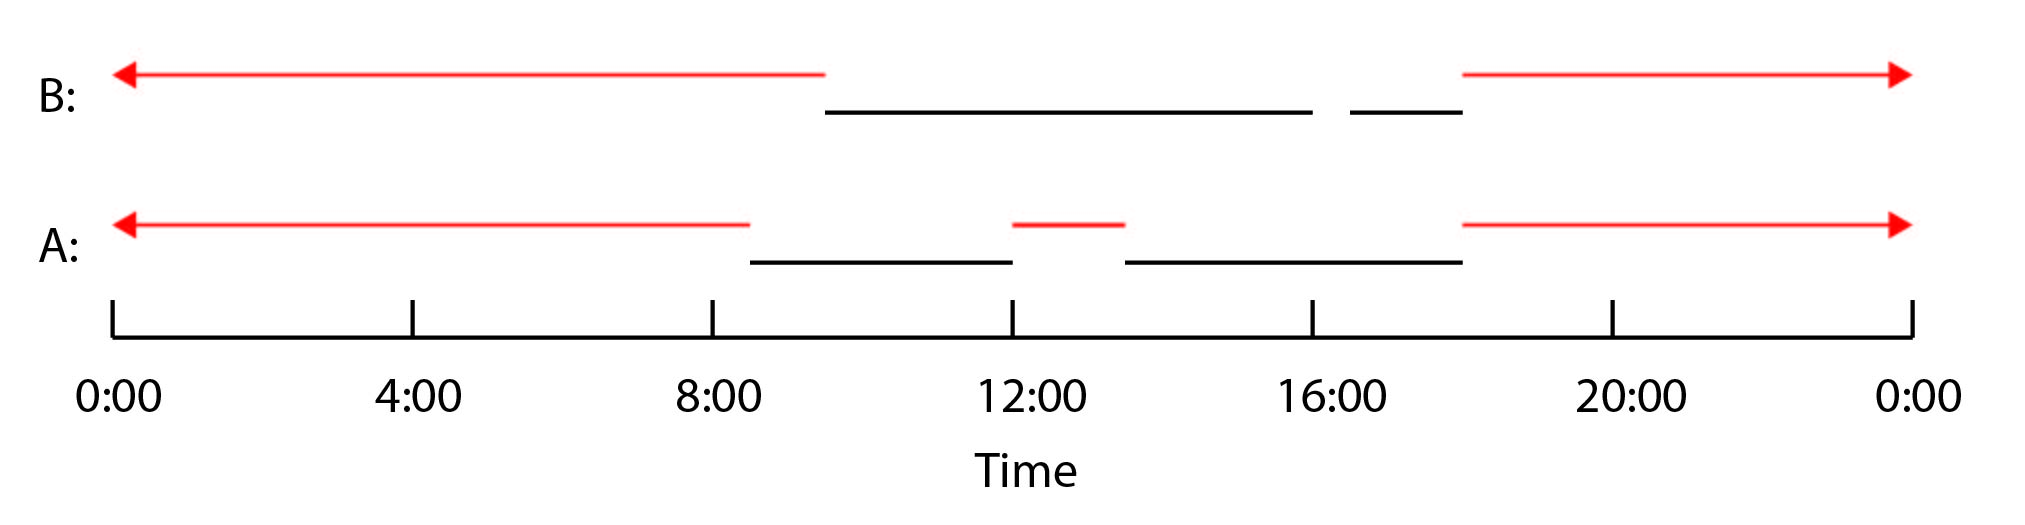
\includegraphics[scale=0.2]{Filling-01}
\captionsetup{justification=centering}
\caption{Filling}
\label{figure:filling}
\end{figure}

\subsection{Grouping}
In order to reduce the data and to be able to filter on people only passing by a building without going in, the data needs to be grouped. The goal is to identify movement patterns between different buildings, this means that records of subsequent scans of the same device in the same building can be grouped together into one single record. The mobile of someone who for example studies the whole day at architecture might have 20 records in the database for that day. This can be reduced to one record that states the time the device arrived at Architecture and left again. To determine whether two records are subsequent in time, and therefore should be grouped together, a threshold for the time gap between two records needs to be defined. As explained in section … the eduroam system has 'scanning rounds' at intervals of 5 minutes and several seconds. If a device is not scanned during a scannig round, but was scanned the round before, the end time of the records is set to the time of the previous scan round plus 5 minutes (see record A1 and B1 \autoref{figure:grouping}). As a result the gap will be a bit more than 10 minutes if someone is not scanned for 2 subsequent rounds (\autoref{figure:grouping} A), and a bit more than 15 minutes if someone is not scanned for 3 subsequent rounds (\autoref{figure:grouping} B). It was decided to set the gap threshold or grouping to 15 minutes. The reasoning behind this is that someone who is not scanned for 3 subsequent rounds has likely left the building. For the example this means records A1 and A2 would be grouped together, records B1 and B2 on the other hand are not grouped.

\begin{figure}[H]
\centering
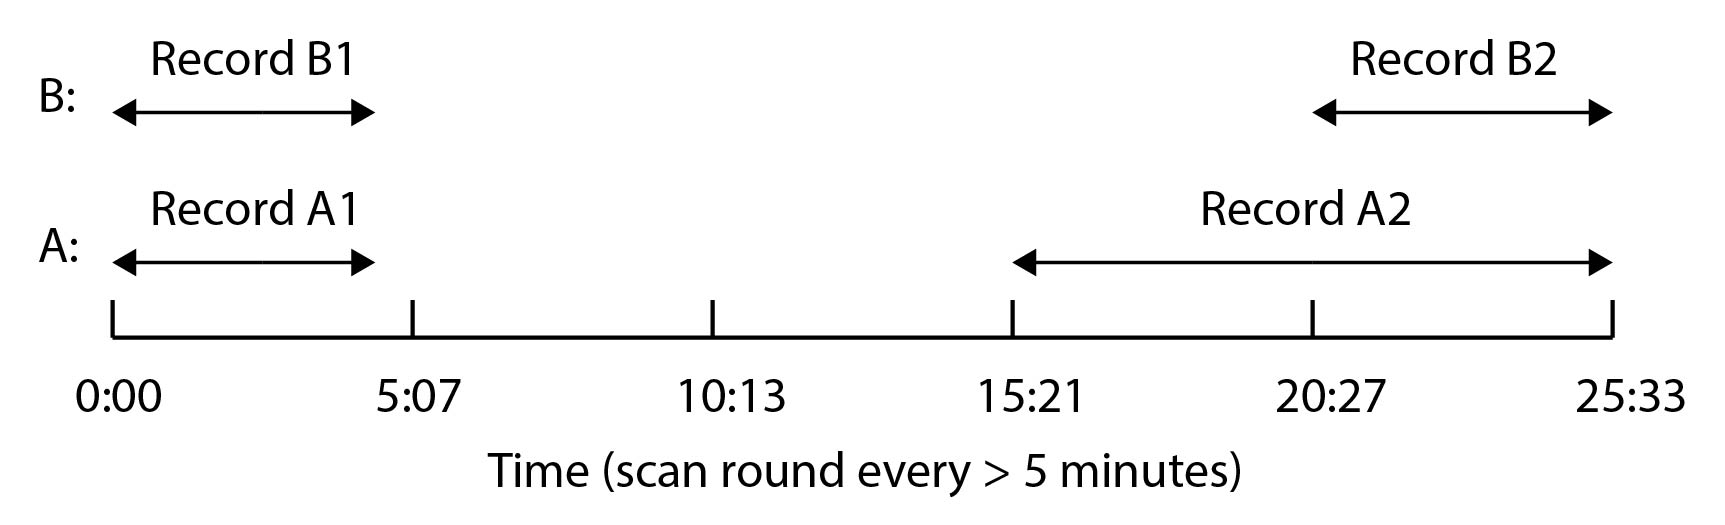
\includegraphics[scale=0.2]{grouping-01}
\captionsetup{justification=centering}
\caption{Grouping}
\label{figure:grouping}
\end{figure}

\subsection{Filtering}

For the detection of movement patterns between buildings, records of people that only pass by a building without actually visiting it should be excluded. The reason for this is that records of people only passing by a building could result in misinterpretation of the movement patterns. If faculty B is for example located on the route from faculty A to the lunch facility. Then it is likely that people moving from faculty A to the lunch facility are picked up by a scanner located at faculty B. As a result the movement from faculty A to the lunch facility will be visualized via faculty B (see \autoref{figure:passing by} top). Someone that isn’t aware of the 'passing by' problem might conclude that people from faculty B make most use of the lunch facility. In reality however, people from faculty A make more use of the lunch facility. By filtering out the records of people only passing by buildings the correct movement can be visualized (see \autoref{figure:passing by} bottom). It should be noted that filtering out 'passing by' records can only be done after the grouping process. The reason for this is that 5-minute records that would individually be classified as someone passing by might be grouped together. After grouping the combined record is not classified as someone who passes by. Furthermore it should be noted that the filtering of 'passing by' records occurs after filling the data with 'world' records. The reason for this that a passing by event does mean that the device was located on the campus. The world records are meant to represent the time the device is not on the campus.

\begin{figure}[H]
\centering
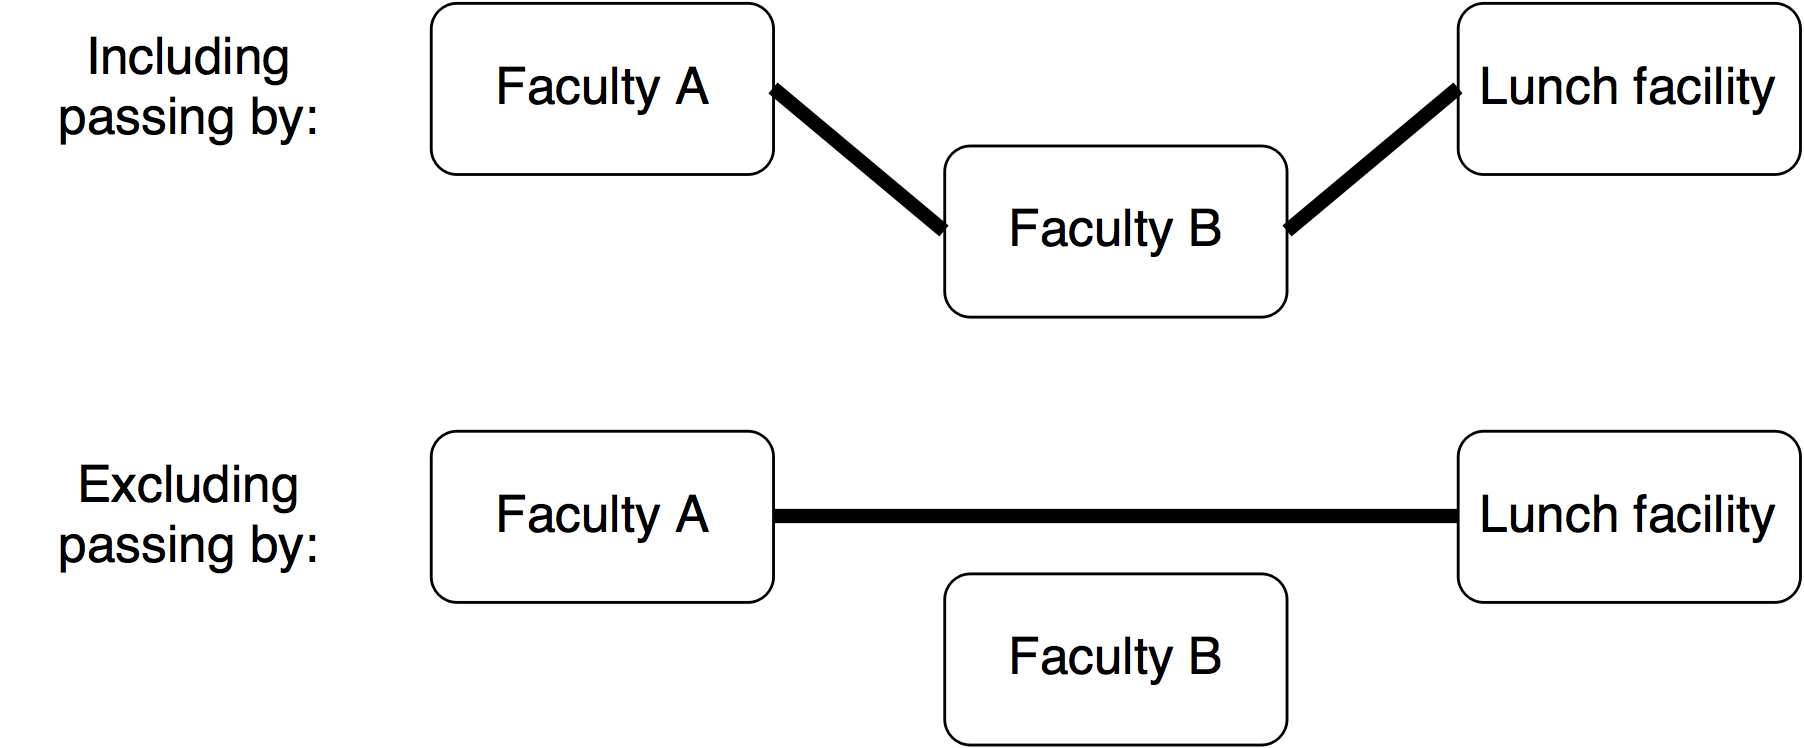
\includegraphics[scale=0.2]{PassingBy}
\captionsetup{justification=centering}
\caption{filtering(Passing by)}
\label{figure:passing by}
\end{figure}
\subsection{Apname vs maploc}
The data in the table 'wifilog' contains information about the location of the Access Point (AP) in two columns. The first one is the column 'apname', which is a string with the symbolic name of the AP, for example 'A-08-G-010'. The two numbers in the second part of the string, in this case '08', represent the building number. This building number can be linked to a location in the world. 
The second column which contains information about location, is the column 'maploc'. This column also contains strings, which look as follows:

System Campus $>$ [buildingid] $>$ [specific location]'. An example of such a string is 'System Campus $>$ 21-BTUD $>$ 1e verdieping'. In such a string, the middle part can be linked to a building, so to a real-world location. 
But there are some other values for maploc, which can less clearly be linked to a real-world location. Such a value is 'Root Area', it is unclear what this value means and it contains no information about a building or area it might be in. This makes it impossible to link it to a location in the world. Then there is the value 'Unknown', a value that indicates that there was no name attached to the Access Point that user was connected to. Again in this case, it is impossible to link this value to a real-world location. 

As both 'Root Area' and 'Unknown' are in the minority of records, they could be left out of the queries. But for some records, the column 'apname' did provide information about the location, while the 'maploc' column value was 'Root Area'. In most of these cases however, the building number, the second part of the string, was a number of length three. But there are no buildings on the TU Delft campus with a building number that high. When consulting Wilko Quack about this, he explained that these building numbers had an arbitrary 1 in front of the building number. So 'A-134-A-001' was not building 134, but building 34, which was an actual building number on the campus. This would mean that using the column 'apname' for getting the building number would mean a higher number of results and therefore a more realistic visualization of the movements. 

Taking the substring of that column and linking it to a building with an actual location is done in two steps. First the whole string is retrieved and with a function in Python the substring is derived. Subsequently, the building id that is the result of this function can be linked to a table in the database which has for every building five columns: buildingid, name, point (as geometry), x (longitude), y (latitude) (see in \autoref{maps}).
\section{Movement between buildings}\label{movement between buildings}
To automate the workflow of creating movement visualizations between buildings, a program is created. There is a distinction between two types of visualization:
\begin{enumerate}
\item Maps
\item Bar charts
\end{enumerate}
The bar plot visualizes the movement throughout the day in 24 bars. Each bar represents the movement from a selection of buildings to another selection of buildings, over a time interval of one hour. In \autoref{barcharts}, the bar charts will be discussed in more detail. For map visualization the JavaScript Leaflet.js is used, this allows for creation of an interactive user interface with a base map from Open Street Maps and visualize the buildings and movement between them. In \autoref{maps} the map visualization will be discussed in more detail. For the bar charts the Python module matplotlib was used.
\subsection{Create movement records}

The data resulting from pre-processing contains the states of where a particular device was located during a certain time period. Implicitly this also includes information on the movement of the device. If a device is first located in building A and subsequently in building B it must have moved from building A to B. However, in order to be able to retrieve the movement patterns of devices the movement should be stored explicitly. This means that each record should store the movement of one device from one building to another building or to world. Examples of movement patterns that can be retrieved from this data are: the number of devices moving from building A to B within a given time period, and the peak in movement from building A to all other buildings. 
\\\\
To create records for each movement first the preprocessed data is ordered on mac address and start time. By doing this all the subsequent states for every device are listed directly below each other (see \autoref{figure:movementrecs}). As a movement is defined by the change of one state to another, movements records can be created from every two consecutive state records (see \autoref{figure:movementrecs}. However, not every two consecutive states represent a movement. Only when the two states concern the same device and they are at different buildings they represent a movement. This means that movement records with different mac addresses or similar building id’s are filtered out (see \autoref{figure:movementrecs}.\\

\begin{figure}[H]
\centering
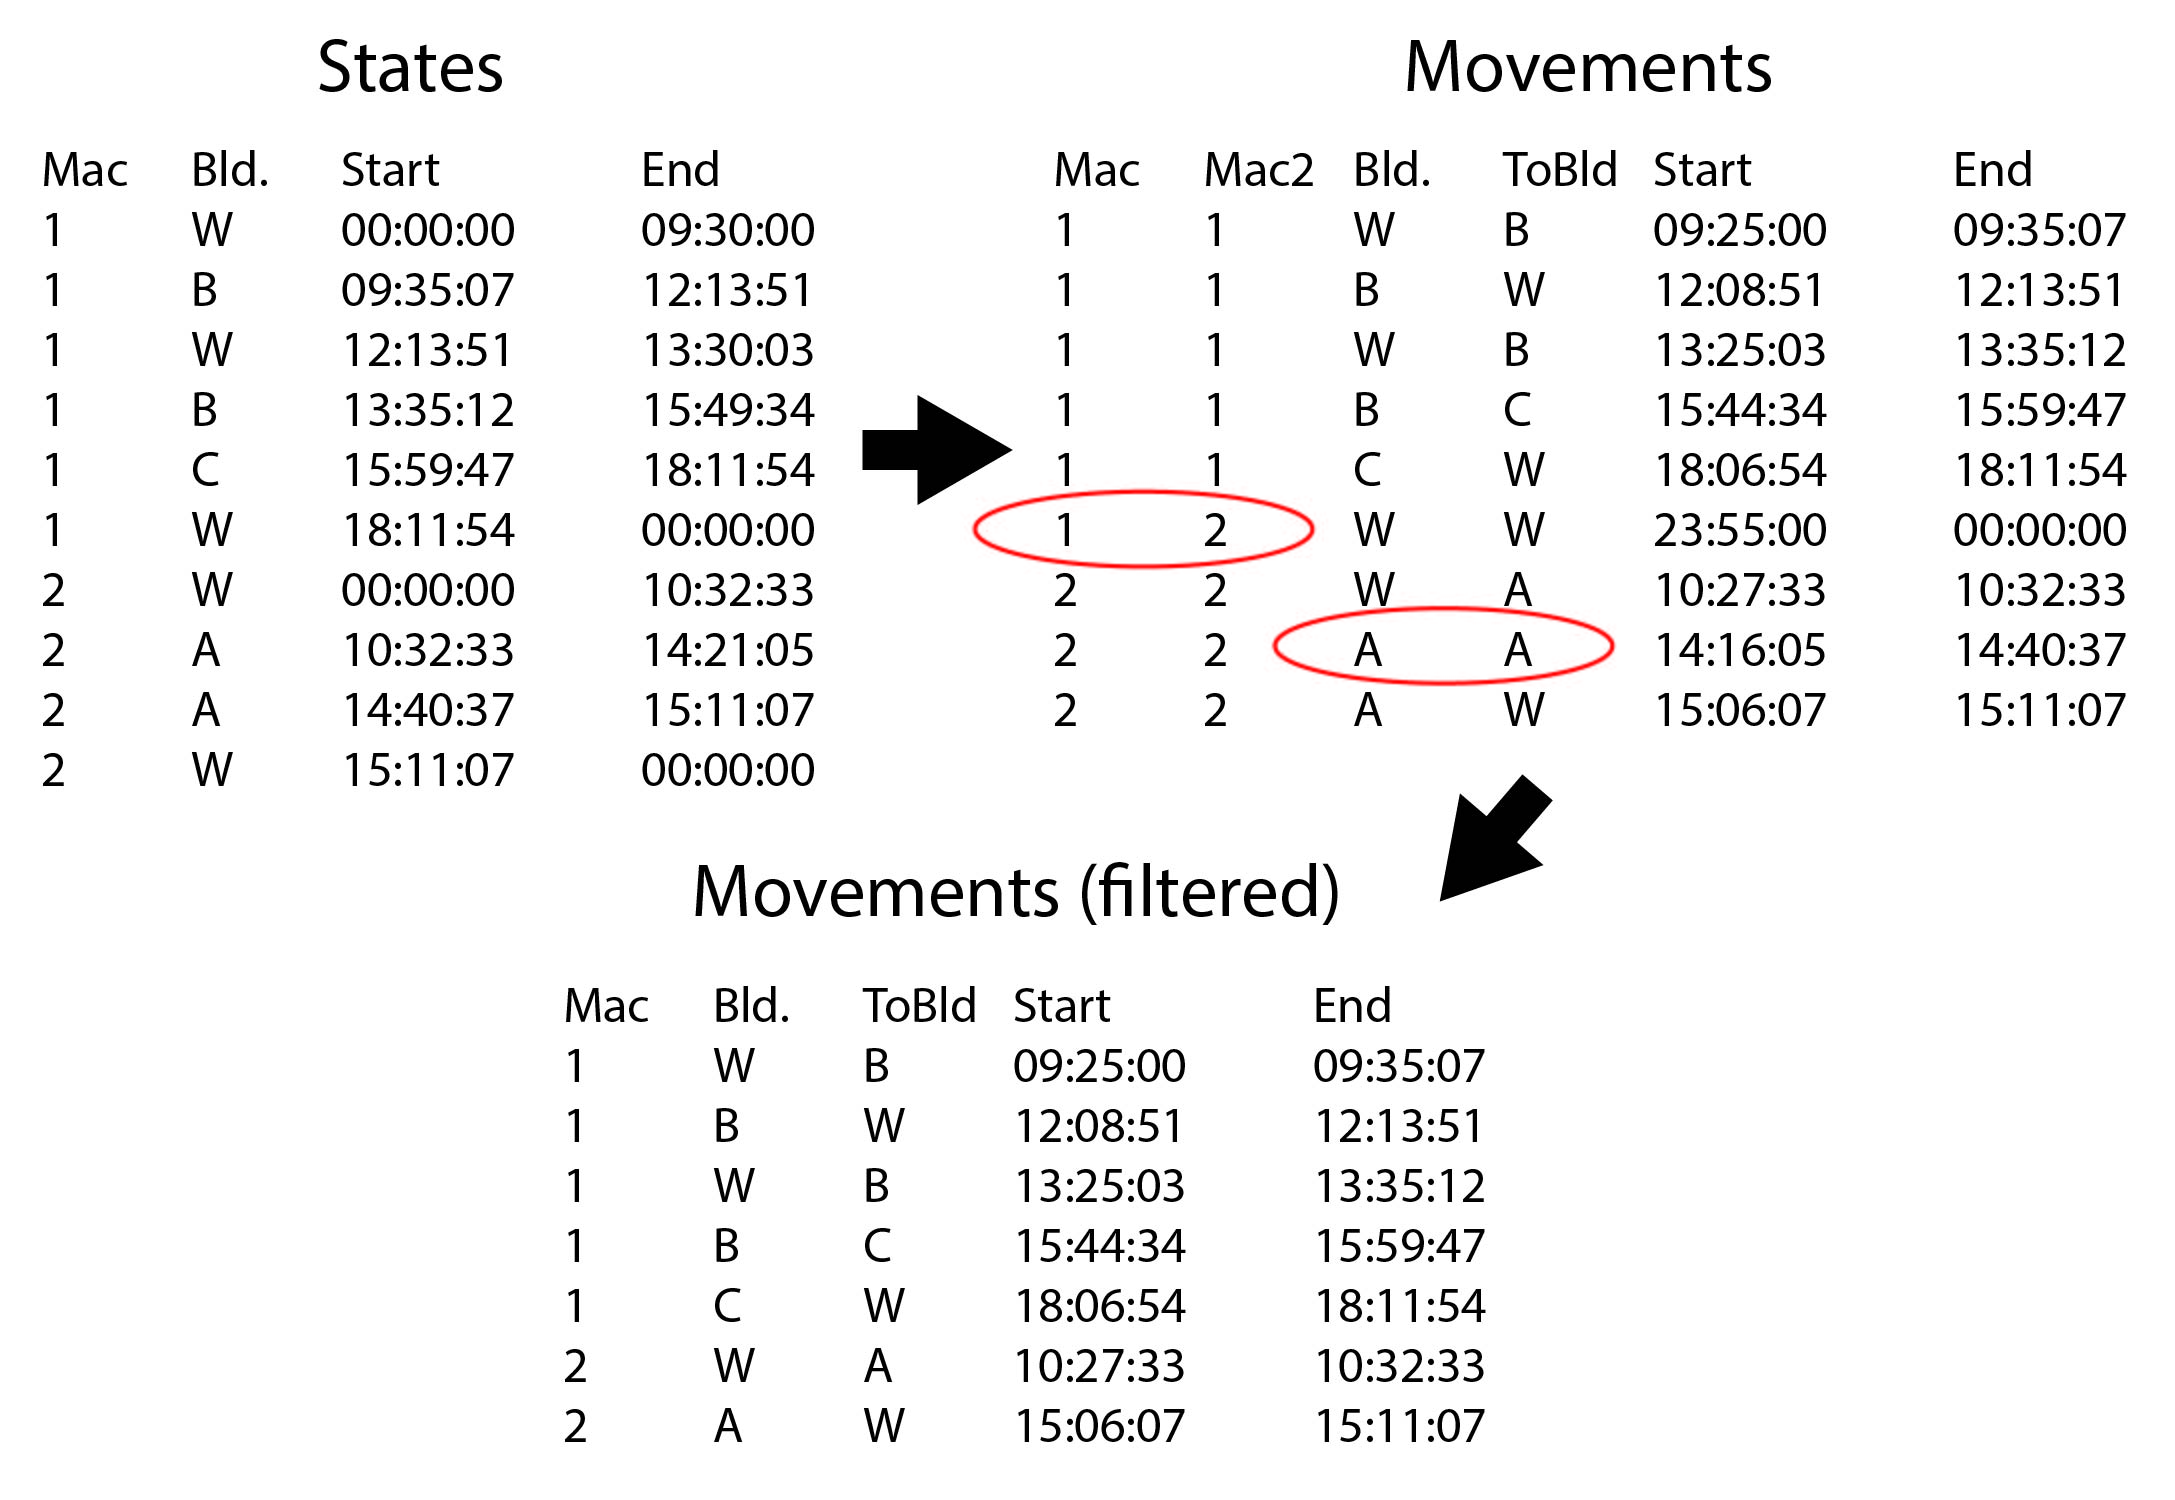
\includegraphics[scale=0.2]{movement_records.jpg}
\captionsetup{justification=centering}
\caption{Movement records}
\label{figure:movementrecs}
\end{figure}

The start and end time of the movement are defined by the end time of the previous state minus 5 minutes, and the start time of the next state (see \autoref{movement}). The reason that 5 minutes are subtracted from the end time of the previous state is that this is approximately the last moment in time the device was actually scanned at the location of the previous state. In the figure below the device is scanned 15:21 at building B. Approximately 5 minutes later (at 20:27) the device is scanned at building C. The state record of building B however continues all the way until 20:27, whilst the last time it was actually scanned at building B was 15:21. As a result it can be concluded that the movement from building B to C took place somewhere between 15:21 and 20:27. Therefore the start time of the movement between B and C can be approximated by subtracting 5 minutes from the end time of the state record at B. As can be observed in the movement from A to B is retrieved in the same way.

\begin{figure}[H]
\centering
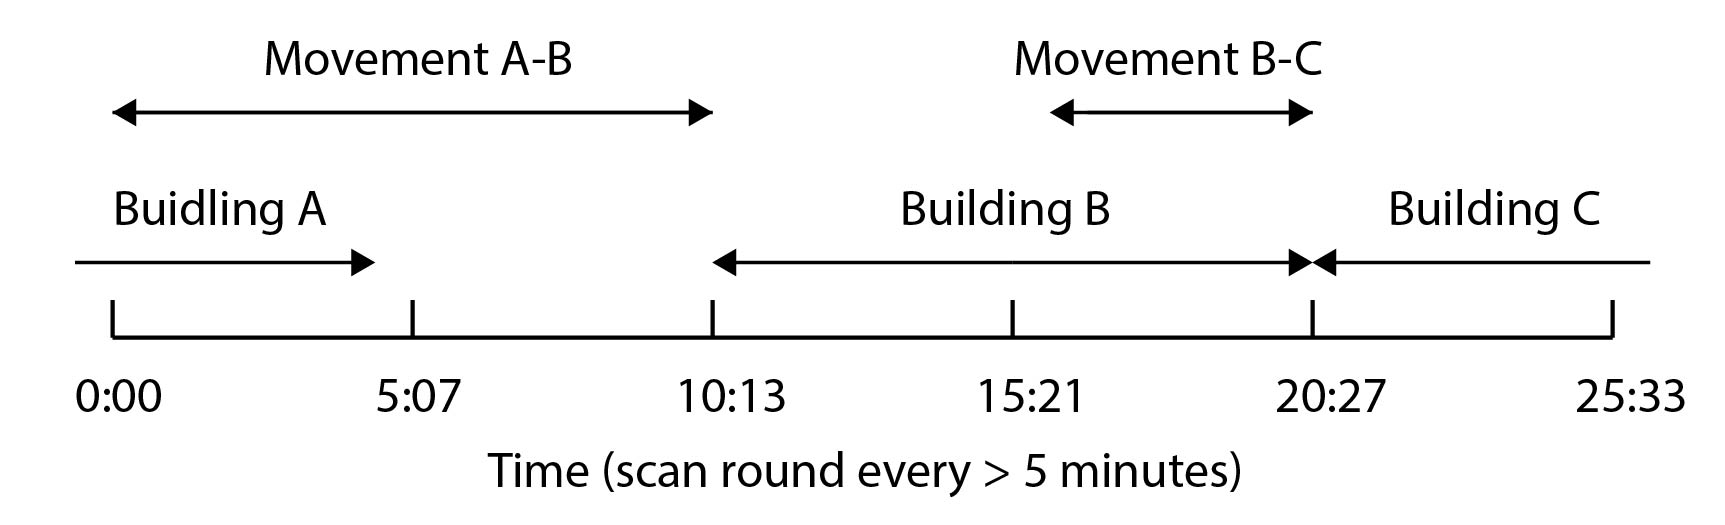
\includegraphics[scale=0.2]{movement.jpg}
\captionsetup{justification=centering}
\caption{Movement}
\label{figure:movement}
\end{figure}


\subsection{Movement over time}

As the described in section \autoref{GUI} the GUI allows a user to select particular days and specify origin and destination buildings of the movement. Based on this input the movement table can be filtered. Finally the filtered data can be visualized as the amount of movement between the specified buildings at each hour of the day. If the user has specified multiple days, the average amount of movement of these days is taken. It should be noted that the amount of movement is defined by the number of devices moving between the specified buildings. \autoref{figure:weekdays_2} gives an example of the visualization of movement over time.
\begin{figure}[H]
\centering
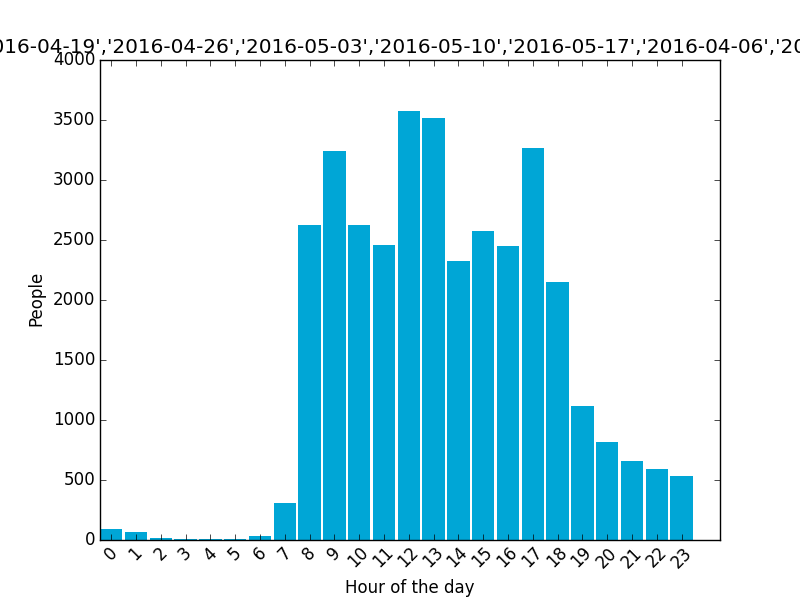
\includegraphics[scale=0.5]{12_weekdays.png}
\captionsetup{justification=centering}
\caption{Movement overtime}
\label{figure:weekdays_2}
\end{figure}


\subsection{Graphical User Interface}\label{GUI}
The Graphical User Interface (hereinafter referred to as GUI) for this work is a Python program that shows a Tkinter interface. When the user runs the program, it will display a main window, which is shown in \autoref{figure:GUImain}
\begin{figure}[H]
\centering
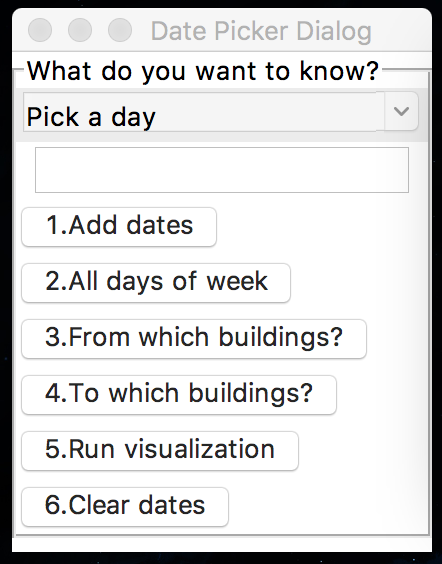
\includegraphics[scale=0.7]{GUI-main}
\captionsetup{justification=centering}
\caption{main window of GUI}
\label{figure:GUImain}
\end{figure}
\pagebreak 
To create a visualization, the user first has to select a time interval and then the buildings from and to which the movement should be visualized. The user has 2 options to select the time series for the current visualization:
\begin{enumerate}
\item Click on '1. Add dates' which will open the date picker dialog
\item Pick a day from the dropdown menu and click on '2. All days of week' 
\end{enumerate}

\begin{figure}[H]
\centering
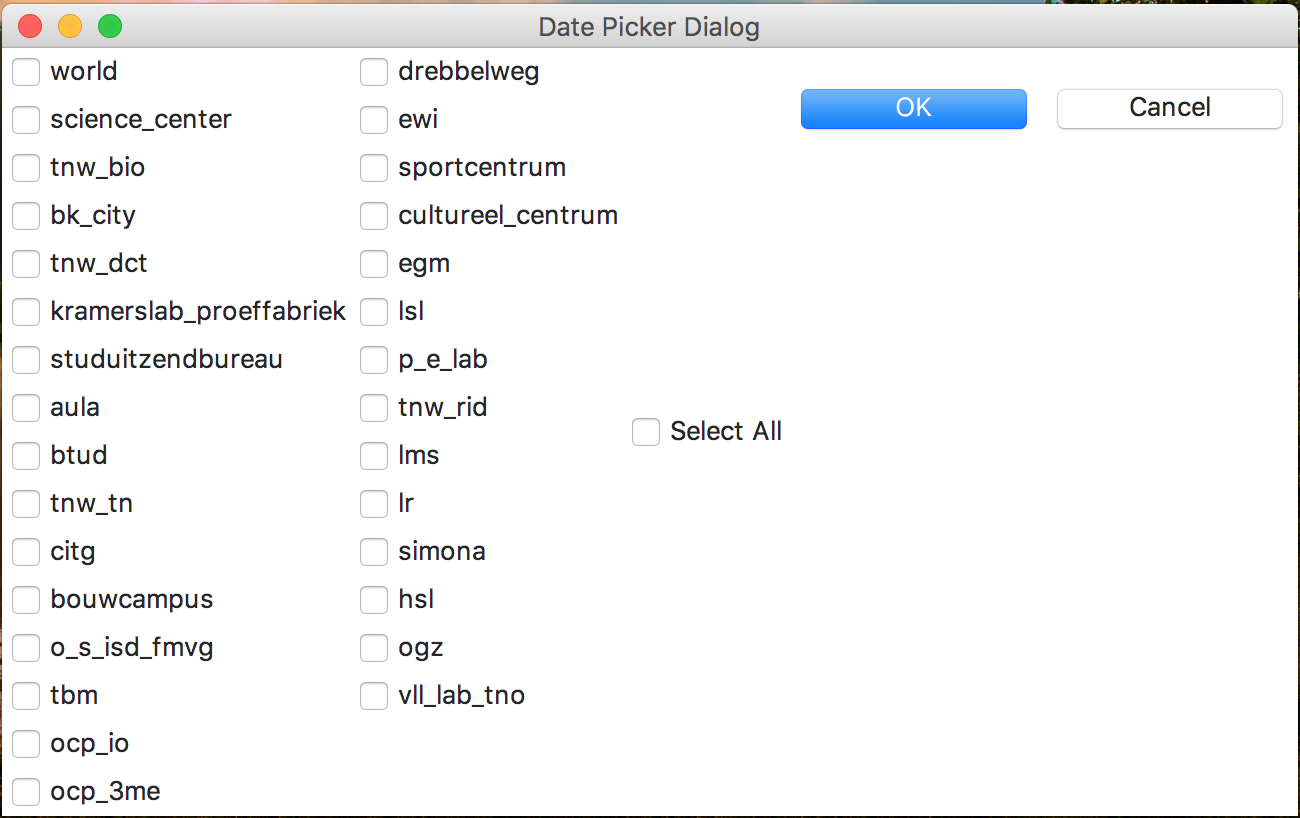
\includegraphics[scale=0.5]{GUI-buildings}
\captionsetup{justification=centering}
\caption{Buildings selection}
\label{figure:GUIbuildings}
\end{figure}

\begin{figure}[H]
\centering
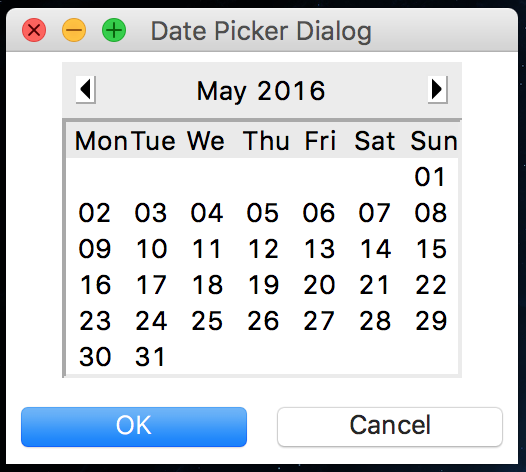
\includegraphics[scale=0.7]{GUI-dates}
\captionsetup{justification=centering}
\caption{Dates selection}
\label{figure:GUIdates}
\end{figure}

Option 1 can be used to select particular days without order. Option 2 can select 'every Tuesday' or even multiple recurring dates, such as 'every Monday to Friday'. It is also possible to combine option 1 and 2 to have for example 'every Monday and Friday the 13th of May'. 

After selecting the time series, the user has to select the buildings from and to which the movement should be visualized. The 3rd and 4th button bring up the same dialog. This dialog shows checkboxes for every building. Every building that is check will be visualized. The user also has the option to select all buildings. If the user would like to see movement from and to the same building, the user can select the same buildings twice.

\subsection{Maps}\label{maps}
In order to get an overview about how people move on the campus and further more,  find out movement patterns, a map visualization is essential. Map visualization consists of three parts: 
\begin{enumerate}
\item base map: open street map is used as a base map. There are many labels on open street map, providing more context of the environment, so it is more clear and readable compared to other base maps like satellite images.
\item building markers: building markers show the locations of the buildings. Google maps marker style is used since it is commonly used in many map application. Because the shape of the building is not useful in analyzing movement patterns between buildings, each building is regarded as a point instead of a polygon, thus a node in the network, 
\item lines: lines are the most essential part in map visualization, they represent movements between buildings.
\end{enumerate}

In the first stage of map visualization, only base map and lines are taken into consideration, building markers are not shown on the map. The line width represents the amount of movement and movements are aggregated daily regardless of the timestamp of each movement during a day. This map visualization gives an overview of the movements over a day and between which buildings there are the most movements. The following maps show the difference of the amount of movement between April 11th (weekday) and April 17th (weekend).

\begin{figure}[H]
\captionsetup[subfigure]{justification=centering}
    \centering
    \begin{subfigure}[t]{0.5\textwidth}
        \centering
        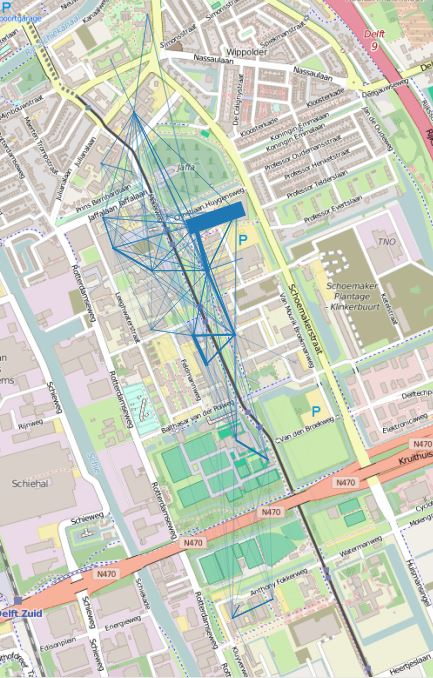
\includegraphics[scale=0.85]{pic1}
        \caption{April 11th, weekday}
    \end{subfigure}%
    ~ 
    \begin{subfigure}[t]{0.5\textwidth}
        \centering
        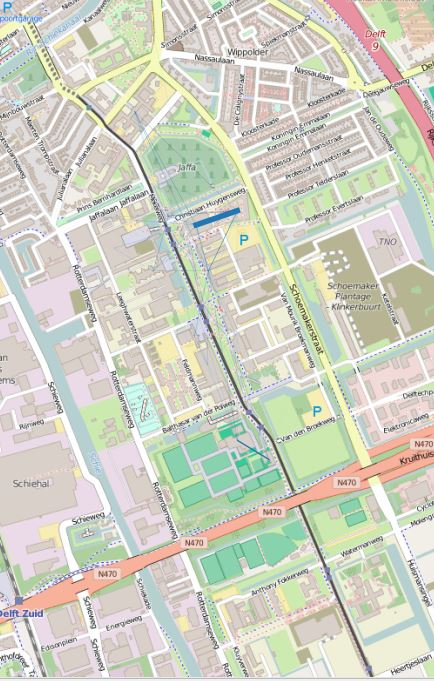
\includegraphics[scale=0.85]{pic2}
        \caption{April 17th, weekend}
    \end{subfigure}
    \captionsetup{justification=centering}
    \caption{Static visualization}
    \label{staticvisualization}
\end{figure}

It's clear that between Aula and library, there are the most movements and the amount of movements is totally different on weekday and on weekend.

Given that movements are dynamic and occuring in both space and time, a dynamic map visualization is created to display individual movement over a day with temporal information. The following screenshots of the gif file show how the movements look like at a certain time of a day:

\begin{figure}[H]
\captionsetup[subfigure]{justification=centering}
    \centering
    \begin{subfigure}[t]{0.3\textwidth}
        \centering
        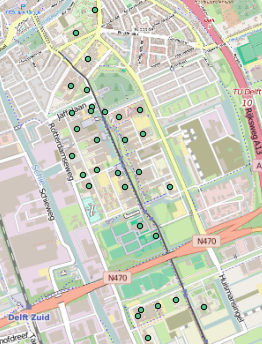
\includegraphics[scale=0.6]{frame009}
        \caption{7:00 am}
    \end{subfigure}%
    ~ 
    \begin{subfigure}[t]{0.3\textwidth}
        \centering
        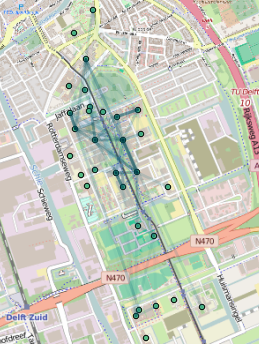
\includegraphics[scale=0.6]{frame021}
        \caption{9:00 am}
    \end{subfigure}
    \begin{subfigure}[t]{0.3\textwidth}
        \centering
        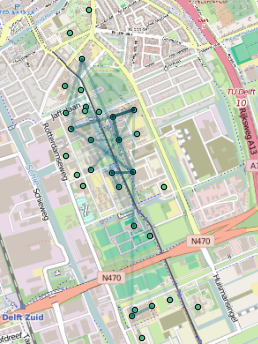
\includegraphics[scale=0.6]{frame033}
        \caption{11:00 am}
    \end{subfigure}
    \begin{subfigure}[t]{0.3\textwidth}
        \centering
        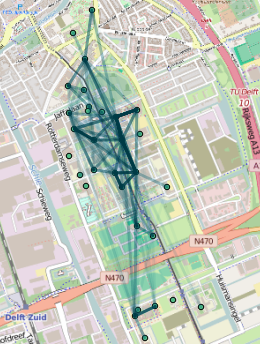
\includegraphics[scale=0.6]{frame045}
        \caption{13:00 pm}
    \end{subfigure}
    \begin{subfigure}[t]{0.3\textwidth}
        \centering
        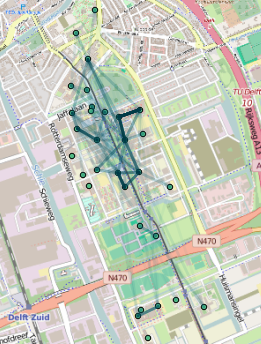
\includegraphics[scale=0.6]{frame057}
        \caption{15:00 pm}
    \end{subfigure}
    \begin{subfigure}[t]{0.3\textwidth}
        \centering
        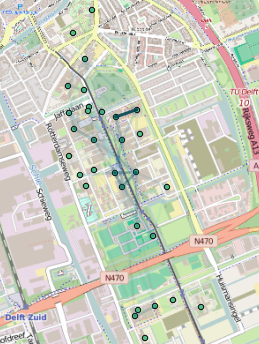
\includegraphics[scale=0.6]{frame066}
        \caption{16:30 pm}
    \end{subfigure}
    \begin{subfigure}[t]{0.3\textwidth}
        \centering
        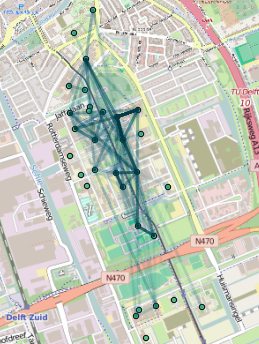
\includegraphics[scale=0.6]{frame075}
        \caption{18:00 pm}
    \end{subfigure}
    \begin{subfigure}[t]{0.3\textwidth}
        \centering
        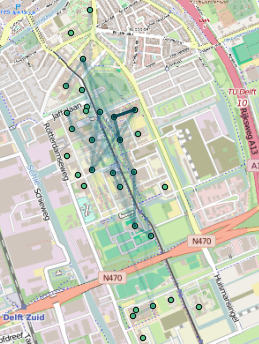
\includegraphics[scale=0.6]{frame087}
        \caption{20:00 pm}
    \end{subfigure}
    \begin{subfigure}[t]{0.3\textwidth}
        \centering
        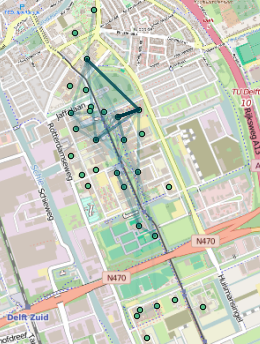
\includegraphics[scale=0.6]{frame099}
        \caption{22:00 pm}
    \end{subfigure}

    \captionsetup{justification=centering}
    \caption{Dynamic visualization of movements, April 11th}
    \label{autovisualization}
\end{figure}

In these pictures, the more movements there are, the less transparent the lines are. So generally speaking, from 7:00 am to 20:00 pm, there are two peaks at 13:00 pm and 18:00 pm. Hence, it is possible to get some insights about movement patterns from the animation. However, the dynamic map visualization doesn't provide detailed information to dig into but only an overview. So in order to find movement patterns, it is necessary to create maps containing more information, including time, direction and so forth. 

Because the amount of data is big, it is more convenient to generate maps automatically so that it will fasten the progress of finding movement patterns. According to the three components of map, there is some information needed to be collected before visualizing movement on map. The locations of buildings are collected manually on Google earth based the campus map. These locations are exported as KML file and imported into QGIS. After adding geometry columns x and y, the csv file is created and imported into database. By using $ST\_MakePoint$ function, a geometry column is created in database. In summary, the building locations are stored as the structure described in following table:

\begin{table}[H]
\centering
\begin{tabular}{|c|c|c|c|c|}
\hline 
id & name & geometry & x & y \\
\hline
0 & world & & & \\
\hline
3 & science\_ center & 010100000042A7.. & 4.36939919846287 & 52.0072322181367 \\
\hline
5 & tnw\_ bio & 010100000043AE.. & 4.37120211221402 & 52.0086132164098 \\
\hline
8 & bk\_ city & 010100000077E3.. & 4.37053698152436 & 52.0056562098059 \\
\hline
12 & tnw\_ dct & 01010000007CA.. & 4.36891378927259 & 52.0040834950037\\
\hline
.. & ... & ....& .... &....\\
\hline	
\end{tabular}
\captionsetup{justification=centering}
\caption{Building data structure}
\label{table:building}
\end{table}

There is a special 'building' called $world$ in the database. It is not an actual location, it is a virtual location which is used if someone is not scanned on the campus in a period of time. After storing the locations of buildings in the database, these locations will be extracted automatically from database to generate maps. There are two properties of lines used to deliver information:
\begin{enumerate}
\item width: line width is used to represent the amount of movements, but the amount is aggregated for both directions.
\item color: color is gradient from red to green. Red line means the movement is not symmetric that much more people move in one direction than the other, while green line means the movement is symmetric.
\end{enumerate}

Based on this map visualization, users can choose certain dates and certain buildings to generate maps automatically. It makes it easier to find out movement patterns. Since not all buildings are chosen, the map will only display the movements between several buildings, which makes the map more readable:
\\\\
\\\\
\\\\
\\\\
\\\\
\\\\

\begin{figure}[H]
	\centering
	\captionsetup[subfigure]{justification=centering}
	\begin{subfigure}[t]{0.48\textwidth}
	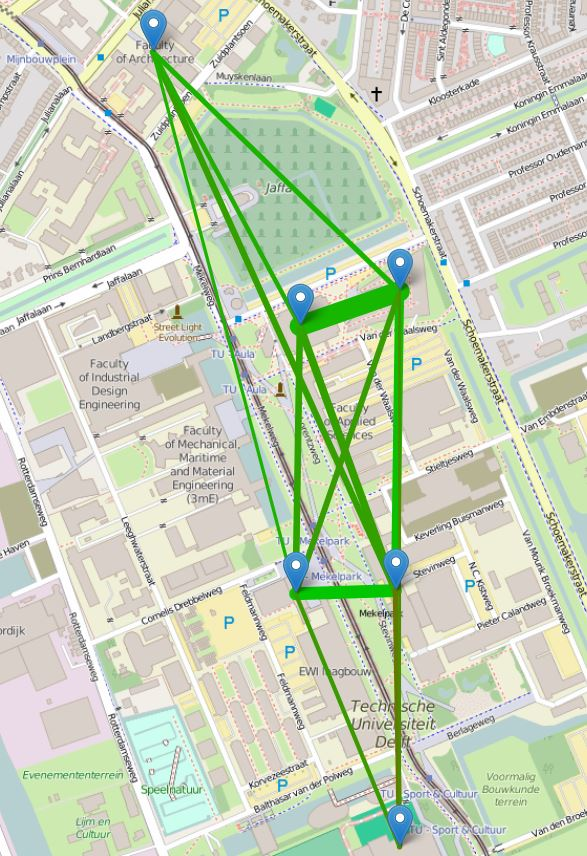
\includegraphics[scale=0.6]{pic3}
	\caption{Amount of movements on April 25th}
	\end{subfigure}
	\begin{subfigure}[t]{0.48\textwidth}
	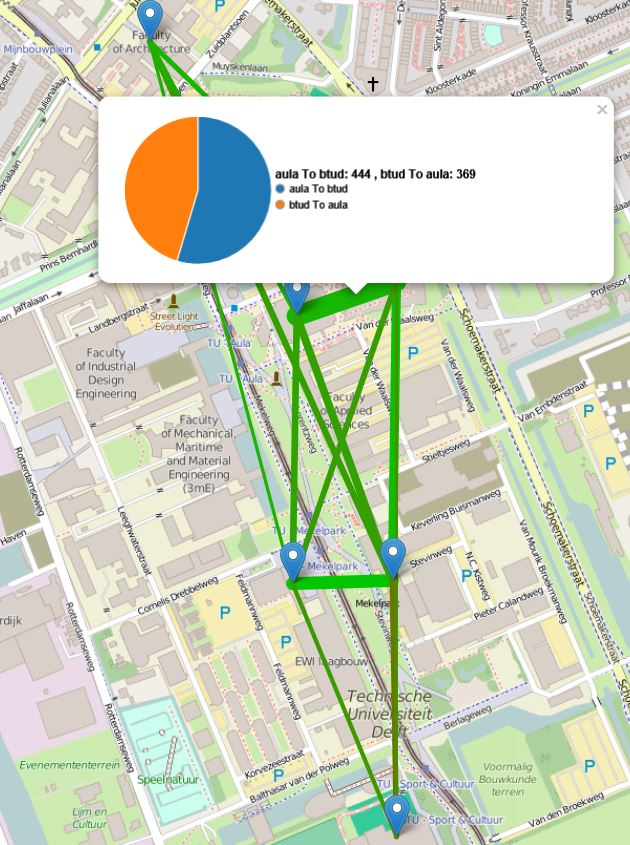
\includegraphics[scale=0.6]{pic4}
	\caption{Amount of movements in pie chart}
	\end{subfigure}
\end{figure}

As shown in the map, the lines are in different colors, which shows the symmetry of the movements. If the user is willing to know more about the movement, it is also possible to click on the line to check the amount of the movements for each direction in detail, and there will be a pie chart showing how symmetric the movements are. With the map visualization, it is easy to focus on movements which are special or interesting.

\section{Trajectories}\label{trajectories}
This GSP attempts to identify people’s movement patterns from anonymized wifilogs. To solve this problem, individual trajectories must be discovered. The data provided by the eduroam network enables a detailed view of people’s movement on campus. The large coverage of the eduroam network allows to track users for a large part of the day when they enter the campus. However, the obeservation space is limited to the extent of the size of the campus, making it not possible to track people outside the eduroam network. A second disadvantage is the spatial resolution of the positioining method. The size of each Wi-Fi cell determines the spatial resolution, as the location of mobile devices is estimated at the origin of a AP. The size of each Wi-Fi cell depends on the distribution of APs. For indoor environments of the TU Delft campus, this is just a few tens of meters wide. This resolution allows tracking movement at a building level by re-locating mobile devices to the closest AP. Data between two re-locations is not available. Therefore, an individual’s trajectory is depicted by connecting the re-locations as a sequence of APs. These individual trajectories are used to identify patterns. 

First, this chapter will describe the extraction of locations of a user. Then the mining of individual trajectories from a anonymized Wi-Fi scanlist is described. Subsequently, the mining of movement patterns in time or space is described. 

\subsection{Location extraction}
A location represents a geographic position where a user stays. For identifying movement patterns from Wi-Fi monitoring, we are interested in movement between two locations where an individual stays for a longer time period. Such a location, or stay place, can be detected when a user is connected to the same AP for a longer time. To detect  buildings as a location (i.e. contains multiple APs), two consecutive WiFi scans must contain  APs of the same building. With a data collecting interval of 5 minutes, it means that people will be filtered out if their stay duration is less than 10 minutes. Based on this assumption, people with a shorter stay duration are considered passing by.

\subsection{Individual trajectory}
An individual’s trajectory is constructed as a sequence of locations in order of the scan time. Start and end time of a trajectory can be specified with a time interval, e.g. a day or week. If p is a location, then a trajectory can be written as:
$$p1 \rightarrow p2 \rightarrow p3 \rightarrow …\rightarrow pn$$

Given a time interval, there is a set of individual trajectories S = \{t1, t2, t3,...,tn\} where each ti is the trajectory over a time interval of one user. 

\subsection{Trajectory Pattern}
From a set S of trajectories, different patterns can be identified using seqeuntial pattern mining algorithms. Frequency of a trajectory by all users of the campus can be detected. This can be represented as a trajactoy T with a support s. Support means how many times the same sequence, or sub-sequence, is shared in the set of trajectories. This gives valuable information on the order common buildings are used and what order of buildings occurs the most. Furthermore, the lenght of a trajectory can be discovered. This allows for identification of movement patterns of a specific lenght n. Also, when location is not considered, but only the lenght of a trajectory, the mobility pattern of an individual can be discribed in terms of how many times he/she re-locates. 

\section{Associated buildings}\label{Associated buildings}

The following section describes how movement patterns were derived on building level, without considering the direction or order of the movement. An association rule mining algorithm (Agrawal et al., 1993) was used to identify groups of buildings that frequently visited in combination with each other. Firstly the algorithm is described briefly, then the results are presented.
\subsection{Association rules mining}
Association rule mining is a technique to analyse what variables or items are commonly associated with each other in large databases. Probably the one of the main application is to analyse which items are commonly bought together by customers of a supermarket. As an example for this use case is an association rule of an itemset \{bread, butter\}, tells that in 80\% of those transactions including \{bread, butter\}, also \{milk\}  was present. In other words, 80\% of the people who buy bread and butter also buy milk (Agrawal et al., 1993). Compared to sequence mining, association rule mining does not consider the order of items neither within, nor across transactions.

Thus every rule is composed by two itemsets, the \textit{antecedent} \{bread,butter\} on the left-hand side, and the \textit{consequent} \{milk\} on the right-hand side. The rule is denoted as \{bread, butter\} \verb|=>| \{milk\}.

\subsection{Assosication rules of buildings}
When a trajectory is simplified into a set of distinct buildings that the person
visited, association rules for buildings can be derived. In this case the rule
describes the set of buildings, or buildingset, that are commonly visited in
combination. For example the rule \{BK\_City, Aula\} \verb|=>| \{Library\}
tells that a group of people who visited the buildings BK\_City and Aula also
visited the Library.

As association rule mining does not consider the order of buildings, nor the
time spent in a building, it is important that these variables are appropriately
handled and noise is filtered out prior running the algorithm.

In the first version the buildingsets were stored in a table as below, where the
field \textit{mac} contains the mac-address of a device and each remaining field
represents a building. Value 1 is given if the device was recorded in a
building, otherwise no value is given. This binary encoding is rather simplistic
as it does not consider the amount of time spent in a building and therefore it
does not allow to differentiate between occasional or regular visits.

\begin{table}[H]
\centering
\captionsetup{justification=centering}
\caption{uncategorized buildingset table}
\label{uncategorized buildingset table}
\begin{tabular}{lllllll}
\cline{1-7}
mac & aula & bk\_city & bouwcampus & btud & ctig & ... \\ \cline{1-7}
A   & 1	& 1    	&        	&  	& 1	& 	\\
B   &  	&      	& 1      	& 1	&  	& 	\\
C   &  	& 1    	&        	&  	& 1	& 	\\
D   & 1	&      	&        	&  	&  	& 	\\
E   & 1	&      	& 1      	&  	&  	& 	\\ \cline{1-7}
\end{tabular}
\end{table}

Therefore in the second version a distinction between \textit{occasional,
regular} and \textit{frequent} stays was added to the buildingsets. The division
between the categories is based on the 40 hour workweek and 1.5 hour lecture
durations (see \autoref{table:stay duration categories}). 

\begin{table}[H]
\centering
\captionsetup{justification=centering}
\caption{Stay duration categories}
\label{table:stay duration categories}
\begin{tabular}{lll}
\cline{1-3}
Category   & hours/week           	& ID \\ \cline{1-3}
occasional & $\leq 0.5$             	& 1  \\
regular	& $\textgreater 0.5, \leq 5$ & 2  \\
frequent   & $\textgreater 5$       	& 3
\end{tabular}
\end{table}

The trajectories of approximately 14,000 devices were used to create the first set of association rules with categorized stay duration. At this stage only the noise was filtered from the data but not the stationary devices, and people carrying two devices were not accounted for. The time range of trajectories spanned from 31.03.2016 to 02.05.2016, approximately one month.

Although there are several measures to evaluate the interestingness of an association rule  (Zhang et al., 2009), only \textit{support} and \textit{confidence} were used for testing purposes. 

\textbf{Support}
“The support for a rule is defined to be the fraction of transaction in the dataset that satisfy the union of items in the consequent and antecedent of the rule.” (Agrawal et al., 1993). In case of the rule \{BK\_City, Aula\} \verb|=>| \{Library\}, the support is the percentage of the total dataset that includes BK\_City, Aula and Library.

\textbf{Confidence}
Confidence measures the strength of the rule, and is considered as a conditional probability. In case of the rule \{BK\_ City, Aula\} \verb|=>| \{Library\}, the confidence is the probability that Library is in the trajectory if both BK\_ City and Aula are in the trajectory (Agrawal et al., 1993; Anbukkarasy \& Sairam, 2013).

The most interesting rules are displayed in \autoref{figure:buildingset}:
\begin{figure}[H]
\centering
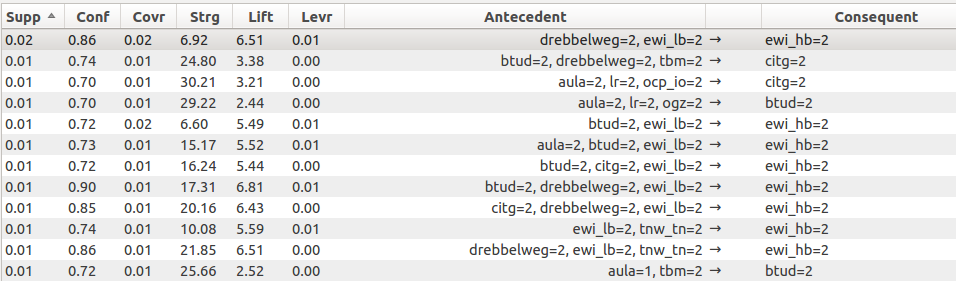
\includegraphics[scale=0.45]{acc_buildingset_v0516}
\captionsetup{justification=centering}
\caption{Building set}
\label{figure:buildingset}
\end{figure}

In the buildingset of approx. 14,000 devices 2\% was recorded in all of the buildings \textit{Drebbelweg, EWI-LB, EWI-HB} (Support = 0.02). There is an 86\% chance that if a device is recorded in the buildings \textit{Drebbelweg, EWI-LB}, then it is also recorded in \textit{EWI-HB} (Confidence = 0.86). And they spent on average between half hour to five hours a week in each building (drebbelweg=2, ewi\_ lb=2, ewi\_ hb=2).

\section{Entrances and exits}\label{entrances and exists}
This section will describe the undergoing process in order to know how frequent the entrances and exits of a building are used. Knowing this will give insight into the use of a building, the spatial context and the relation between these two. Our hypothesis is that access points located near the entrance(s) of a building are most frequently used as first access point when entering a building, and as last access point when leaving a building. Firstly, an approach will be presented that does not take in account that devices might get scanned when passing by the building. In the second approach we will make use of the pre-processed data which excludes the devices that get scanned when passing by the building. 

\subsection{First approach:including devices passing by}
The first approach makes use of the raw wifilog data, by finding the part in a sequence in which a device is scanned by an access point in a building and is subsequently scanned in another building. With the location of the access points known, we hope to get insight into the use of an entrance or exit location in a building. 
\begin{figure}[H]
\centering
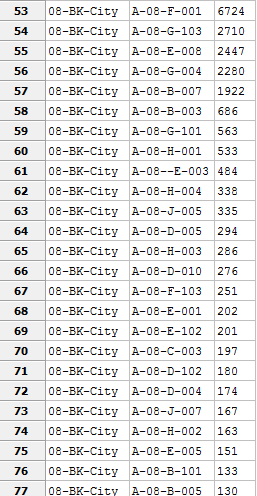
\includegraphics[scale=0.45]{entrances_firstapproach_bk}
\captionsetup{justification=centering}
\caption{A segment of the resulting table after querying}
\label{figure:Entrance1ApproachTable}
\end{figure}

The stays in which the device is scanned once are not filtered out. These single scans imply that a person with the device only passed by the building, thus was not really located in the building. 

\begin{figure}[H]
\centering
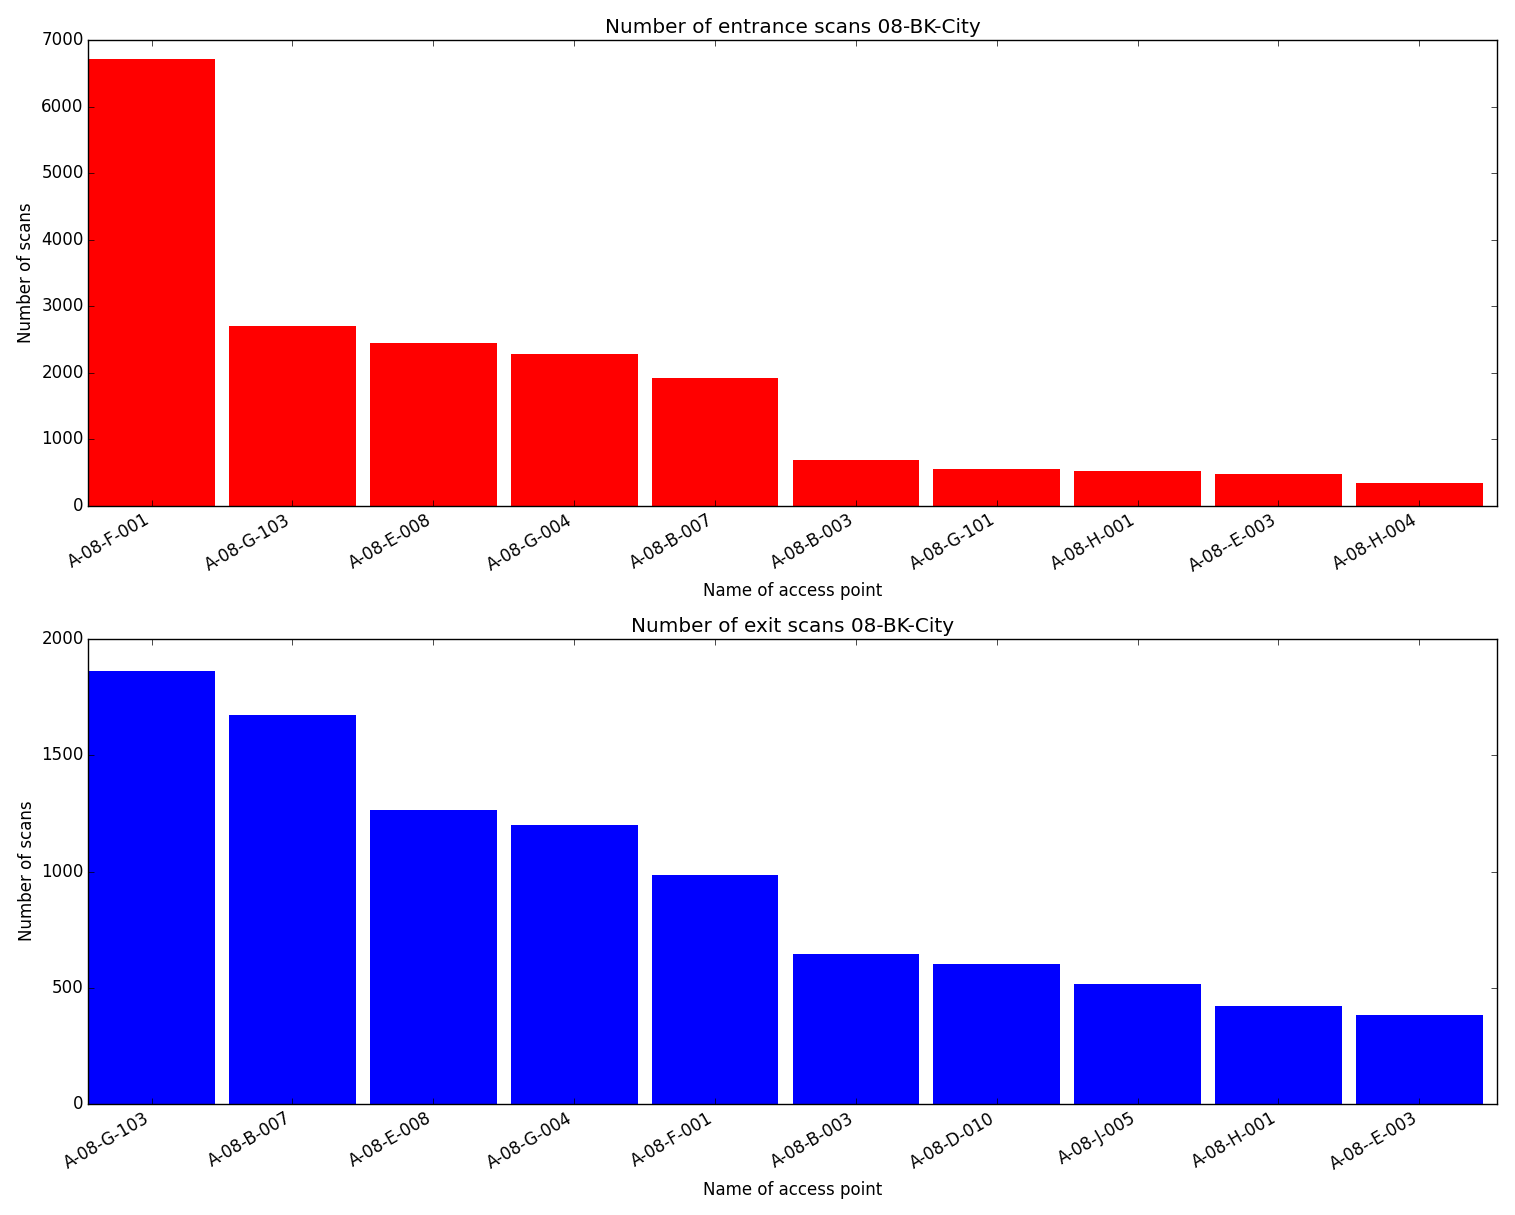
\includegraphics[scale=0.32]{entrances_firstapproach}
\captionsetup{justification=centering}
\caption{Most frequently used entrance and exit access points in BK-City}
\label{figure:Entrance1Approachfigure}
\end{figure}

In order to know whether these access points(see \autoref{figure:Entrance1Approachfigure}) are located near an entrance, the access point maps of BK-City is used. The access point maps are the building plans enriched with the location of each wifi access point installed in the building. Currently, the access point maps of BK-City are the only ones available. Looking at the location of the access points with the highest frequency, gives an interesting result (\autoref{figure:Entrance1Approachaploc}).
 
\begin{figure}[H]
\centering
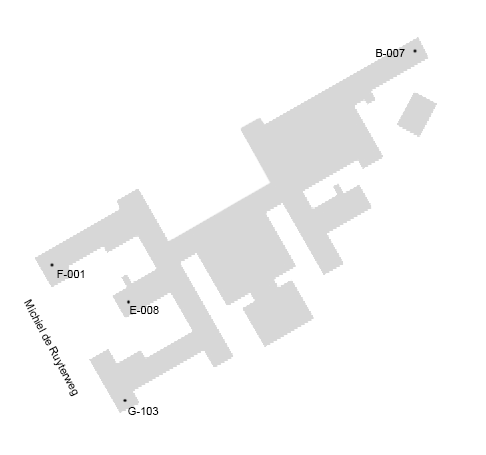
\includegraphics[scale=0.7]{entrances_aplocs_firstapproach}
\captionsetup{justification=centering}
\caption{The location of the most frequently used entrance and exit access points}
\label{figure:Entrance1Approachaploc}
\end{figure}
Most of the frequently used access points are located at the western part of BK-City (\autoref{figure:Entrance1Approachaploc}). Also, there is no entrance or exit located near most of these access points. Knowing that lots of people are passing in the street next to the western part of the building, we can conclude the result of this analysis is distorted due not filtering out the devices that get scanned when passing by the building.

\subsection{Second approach:excluding devices passing by}\label{secondapproach}

\autoref{figure:Entrance2Approachtable} depicts the table as a result of the pre-processing as described in \autoref{preprocessing}. The records represent the stays for each mac, including the first and last access points (ap\_ start and ap\_ end).

\begin{figure}[H]
\centering
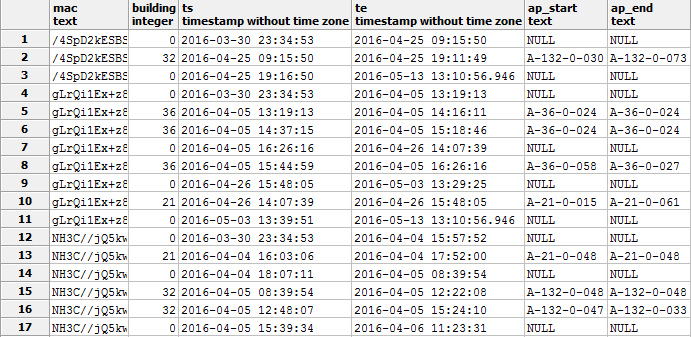
\includegraphics[scale=0.6]{entrances_secondapproach_table}
\captionsetup{justification=centering}
\caption{A segment of the table as a result of the pre-processing}
\label{figure:Entrance2Approachtable}
\end{figure}

The table also includes 'world' (in the \autoref{figure:Entrance2Approachtable} represented by NULL) which implies the device is not located on the campus. 

The following simple SQL statement is used to plots the most frequently used entrance access points.

\begin{lstlisting}[language=SQL]
SELECT ap_start, count(*)
FROM table
GROUP BY ap_start
ORDER BY count desc;
\end{lstlisting}	

Ap\_ end is used, instead of ap\_ start, for plotting the most frequently used exit access points in a building.

\begin{figure}[H]
\centering
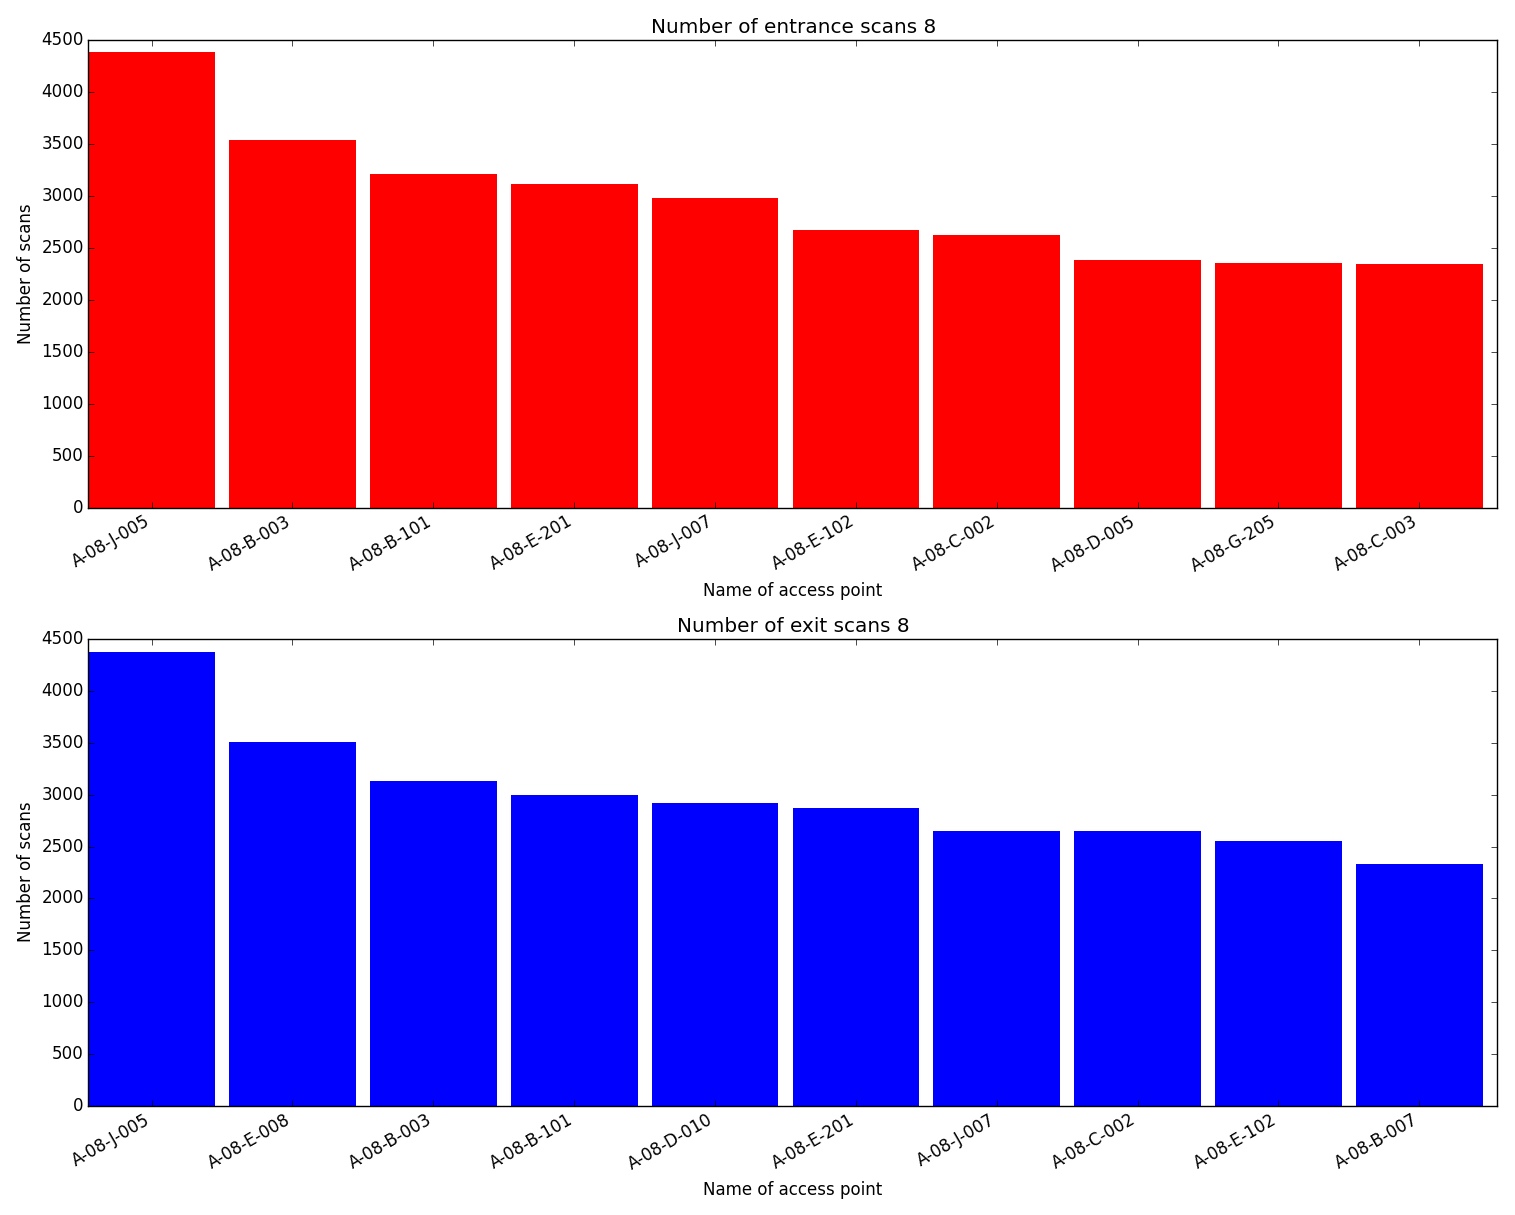
\includegraphics[scale=0.32]{entrances_secondapproach}
\captionsetup{justification=centering}
\caption{The most frequently used entrance and exit access point for BK-City
}
\label{figure:Entrance2Approach}
\end{figure}

The most frequently used access point, A-08-J-005, is not located near an entrance or exit (see \autoref{figure:Entrance2Approach}). This is different than expected. Although it is not very logical in the first place, it still might be one of the first or last access points a device connects with. The reason for this is that the A-08-J-005 access point is placed in in an open space without many objects that could block the wifi signals.

\begin{figure}[H]
\centering

\includegraphics[scale=0.6]{map_ap1_secondapproach}
\captionsetup{justification=centering}
\caption{The location of the most frequently used entrance and exit access point, according to our second approach
}
\label{figure:Entrance2Approachaploc}
\end{figure}

We expected the access point to be located much closer to an entrance or exit. The plan is to set up an experiment in order to justify the unexpected result. In this experiment we will check to what access points different devices (laptops and mobile phones) connect when entering or leaving a building.

\subsection{Frequency of entrance and exit access points}
This section will describe the analysis on the frequency of entrance and exit access points. As described in \autoref{secondapproach}, the most frequently used entrance and exit access points are not always are located near an entrance or exit. Though it is still possible to analyze how frequent these access point are used. The results will be aggregated, meaning it represents more than a single day.

\textbf{Entering}
First we will take a closer look at an access point which appears to be one of the first that scans the device. This will be A-08-J-005 in BK-City, see \autoref{figure:Entrance2Approach} in \autoref{secondapproach}. The chart below shows the frequency of entrance access point A-08-J-005 for devices entering BK-city, over a 24 hour time period. 

\begin{figure}[H]
\centering
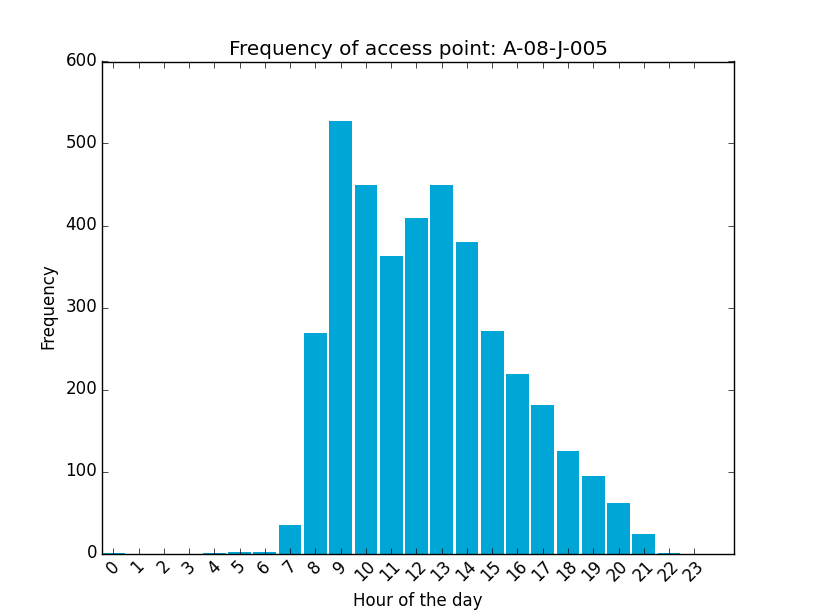
\includegraphics[scale=0.5]{entrances_frequency_secondapproach}
\captionsetup{justification=centering}
\caption{Frequency of entrance access point A-08-J-005
}
\label{figure:A-08-J-005Entrance}
\end{figure}

The chart shows two peaks; in the morning and around 12pm to 1pm. This is in line with what we expected. In the morning a large group enters the building and around 12pm to 1 pm a large group enters the building after the lunch break. 

\textbf{Exiting}

For the exit situation, again the A-08-J-005 access point will be used. This access point also appears to be the most frequently used exit access points. The chart below depicts the frequency of devices leaving the building over a 24 hour period.

\begin{figure}[H]
\centering
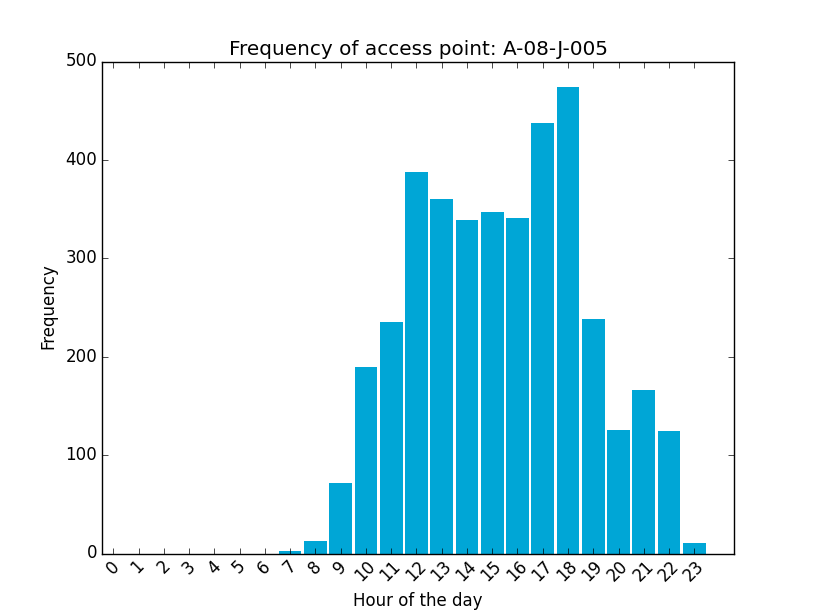
\includegraphics[scale=0.5]{exits_frequency_secondapproach}
\captionsetup{justification=centering}
\caption{Frequency of entrance access point A-08-J-005
}
\label{figure:A-08-J-005Exit}
\end{figure}

The chart shows three interesting peaks, which is in line with what we expected. The first one, around 12am to 1pm, is due the people that leave the building, most probably for lunch. The second peak, around 6pm to 7pm, is due the people that go home for diner. The last one, around 9pm to 10pm, is due the fact the building closing time of the building.

\section{Static and mobile devices}\label{Static and mobile devices}

In order to identify the movement patterns and know what entrances and exits are most frequently used even better, we aim to identify dynamic and static devices. In our first approach, we will look at the number of different access points the device is scanned by in time. The distinction between static and dynamic devices is important, because the behaviour, in terms of Wi-Fi tracking, is significantly different. For instance, a static device, such as a laptop, connects with the Wi-Fi network at different moments compared to a dynamic device, such as a mobile phone. The difference will be explained more in detail using the image below. 

Assume a person that carries a static device (laptop) and a dynamic device (mobile phone) enters a building. While being on his way to the destination, the person does not make use of the laptop, thus the laptop is not connected to the Wi-Fi network. On the other hand, the Wi-Fi of the mobile phone is turned on all the time, and connects at the moment the device is on range of the first access point. On the way the mobile phone is scanned by Access Point(AP) 1, 2 and 3. The person connects to the Wi-Fi network with the laptop at the moment it arrives in the room, of which the Wi-Fi is covered by AP 3. This access point scans the laptop for first time after entering the building. The static laptop is distorting the result, due the fact that in this case the entrance access point for the laptop would be AP 3. In order to achieve a more reliable result, the aim is to filter out the static devices.

To identify the static and dynamic devices, we analyze the behaviour of each device. The first approach focuses on the number of (distinct) access points and the session duration. We assume to find differences between them (\autoref{table:staticanddynamic}). 

\begin{table}[H]
\centering
\begin{tabular}{|c|c|c|}
\hline 
 & Session duration & Nr.of access points \\
\hline
Static & long & low \\
\hline
Dynamic & short & high \\
\hline	
\end{tabular}
\captionsetup{justification=centering}
\caption{Difference between static and dynamic devices}
\label{table:staticanddynamic}
\end{table}

We expect that the relation between the distinct access points and the (summed) session duration, called ratio, is going to be useful in making the distinction between static and dynamic devices (\autoref{equation:staticdynamic}).

\begin{equation}\label{equation:staticdynamic}
Ratio = distinct access point / summed session duration
\end{equation}

In this, a small ratio indicates the device is dynamic and a large ratio indicates the device is static. The result shows that the number of devices decreases over ratio(\autoref{figure:staticanddynamic}).
\begin{figure}[H]
\centering
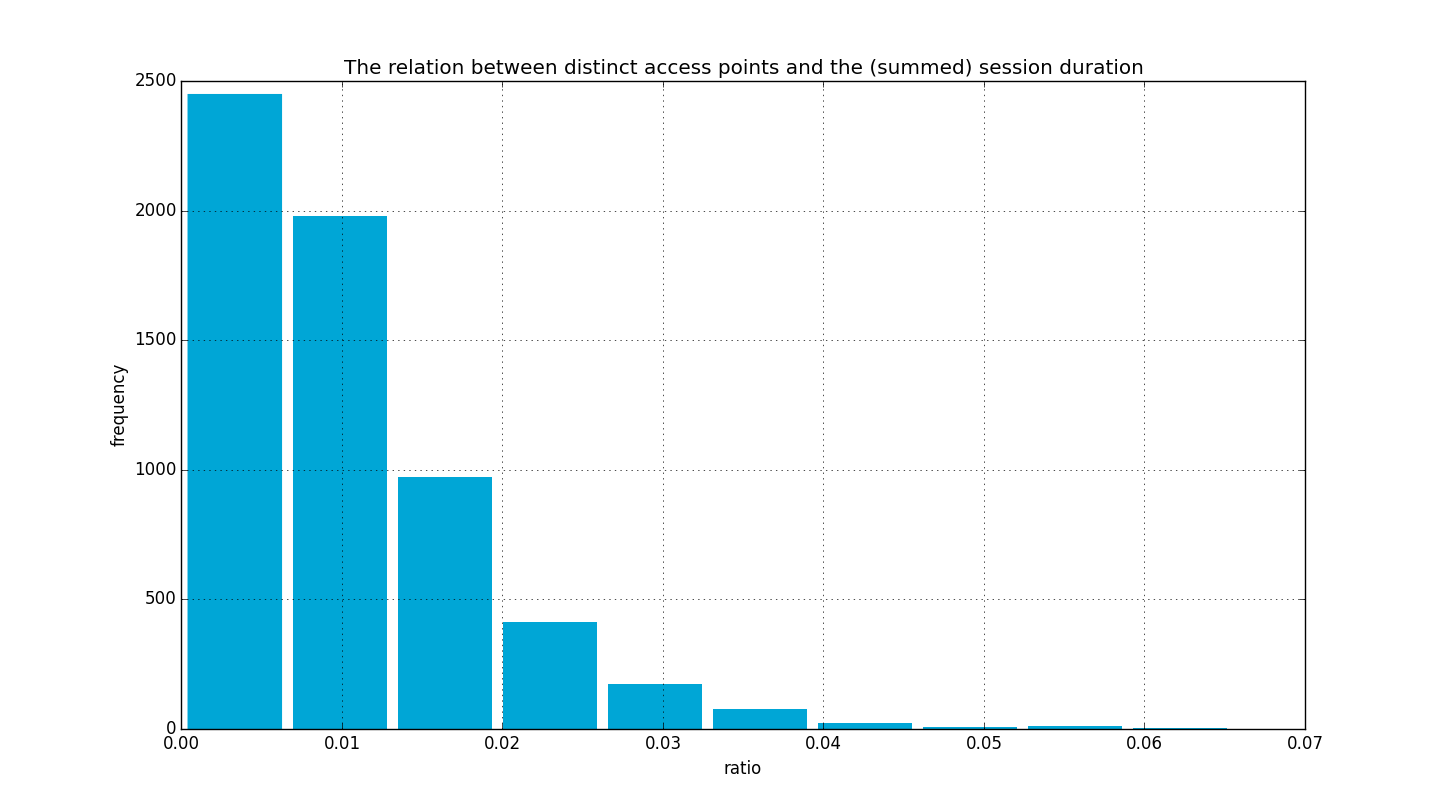
\includegraphics[scale=0.4]{static_vs_dynamic_histogram}
\captionsetup{justification=centering}
\caption{The relation indicating frequency of a radio}
\label{figure:staticanddynamic}
\end{figure}

Because the frequency decreases gradually, there is a fuzzy boundary that separates the static from dynamic devices. Therefore it not (yet) possible to filter out the static devices for further analysis. In order to improve this, the plan is to use the exact number of access points that scanned the device instead of the distinct access points. Also, a closer look will be taken at the session duration, since dynamic devices will have session duration of approximately 5 minutes much more often. 


\section{Preliminary Results}\label{results}

The movement trajectories and the amount of movement between buildings can be visualized in maps and bar charts. The previous sections explained how the data is transformed and this section focusses on the results that can be derived from this data. Bart Valks and Iljoesja Berdrowski stated some questions that arise in their line of work and this section will try to answer these questions with the visualization in both maps and bar charts.
\\\\
\subsection{Movement to the Aula on weekdays}

The department of FMRE would like to know if the faculty of Applied Sciences uses the restaurant facilities of the Aula more than other buildings, due to the fact that the two buildings are connected with a bridge on the first floor.

The graph below shows the average movement of people to the Aula on weekdays. Clearly a peak can be distinguished in the morning between 8:00 and 9:00, around lunch time and in the afternoon between 17:00 and 18:00. The morning and afternoon movements represent people moving from home to the aula and back home.
\begin{figure}[H]
\centering
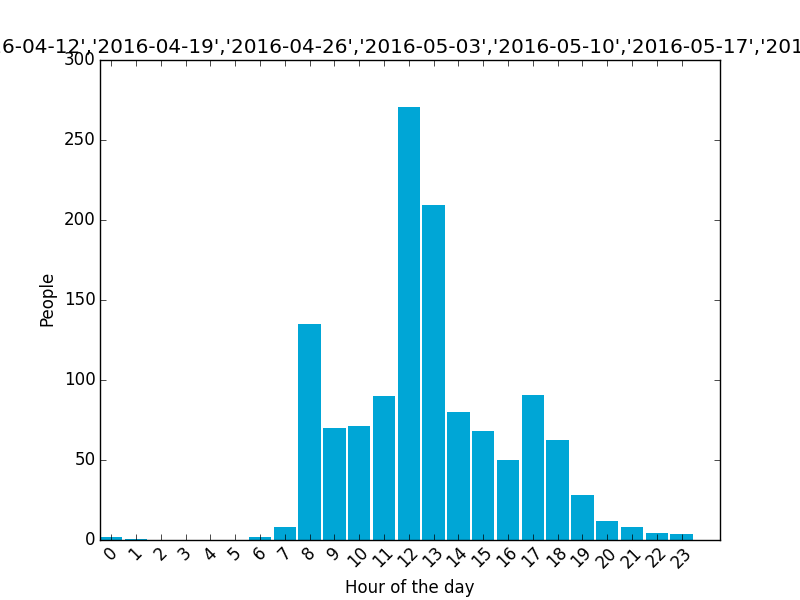
\includegraphics[scale=0.6]{all_to_aula.png}
\captionsetup{justification=centering}
\caption{All to Aula}
\label{figure:all to aula}
\end{figure}

The graph however, says nothing about which buildings contribute the most to the movement to the aula. The map image below shows the top 10 buildings with movement to the aula. It is clear that most of the movement comes from the Library. But if leaving the Library out of the equation, it is clear to conclude that the faculty of Applied Sciences uses the aula more than other faculties. The movement from TNW to the aula is 5000 people over the whole dataset, where other faculties don’t get higher amounts than 2500. 

\begin{figure}[H]
\centering
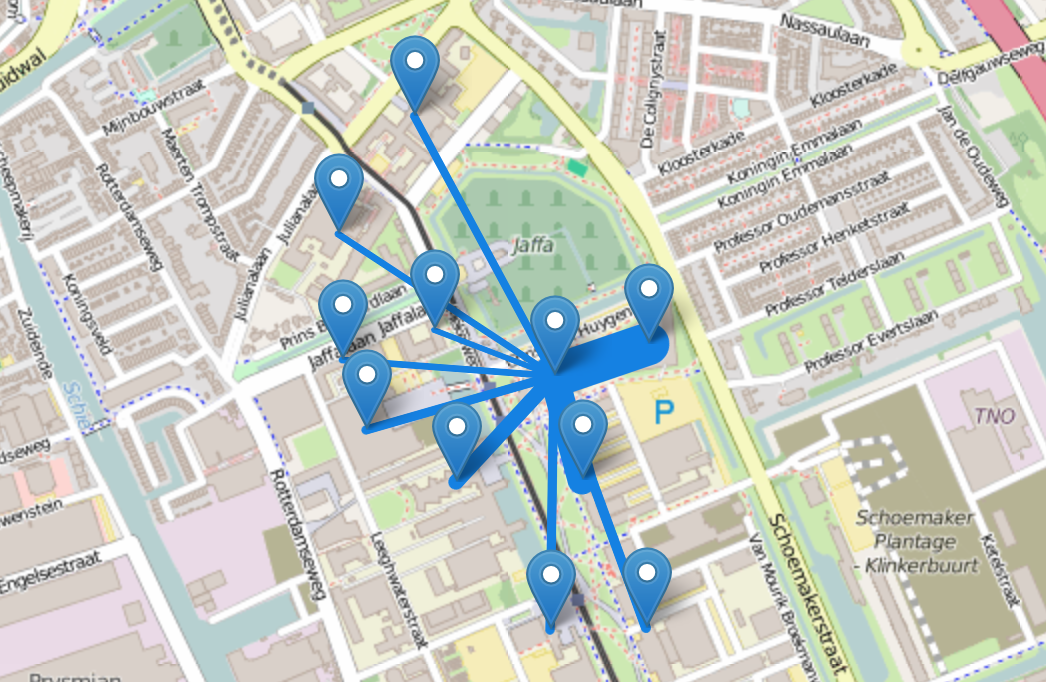
\includegraphics[scale=0.65]{map_all_to_aula.png}
\captionsetup{justification=centering}
\caption{Maps from all buildings to Aula}
\label{figure:all to aula maps}
\end{figure}

This partly confirms the assumption that FMRE made, but to be sure, the movement from the faculty of Applied Sciences must also be checked, in order to see if the movement to the aula is no exception. The result of this visualization is shown in the map image below.

\begin{figure}[H]
\centering
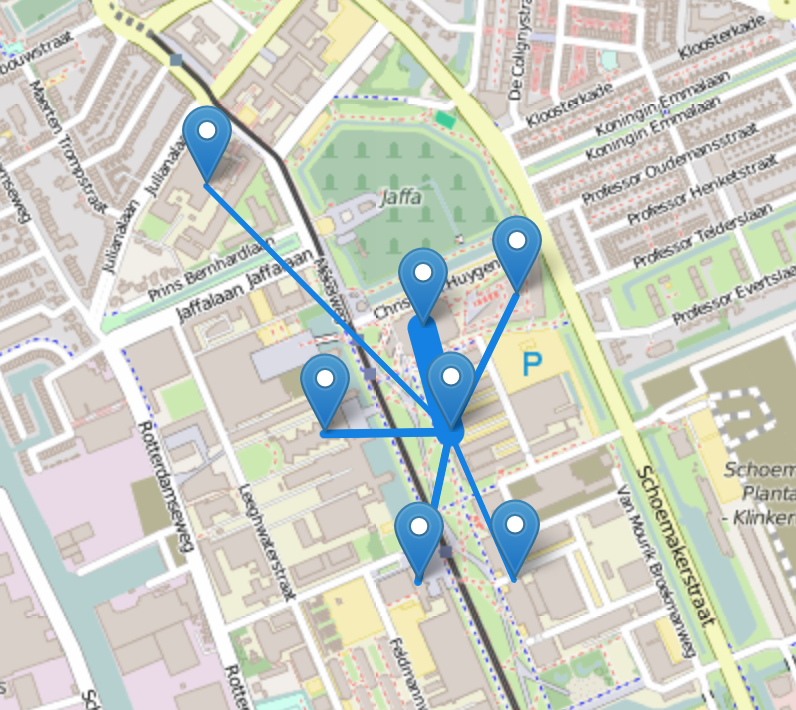
\includegraphics[scale=0.7]{map_all_to_tnw.png}
\captionsetup{justification=centering}
\caption{Maps from all buildings to TNW}
\label{figure:all to TNW maps}
\end{figure} 

This image shows that indeed most of the movement originating from the faculty of Applied Sciences is going to the Aula. The bar chart provides more insight in when this movement is taking place, which is during lunch, as expected. 
\\\\
\subsection{Movement on weekdays vs. weekends}
\begin{figure}[H]
	\centering
	\captionsetup[subfigure]{justification=centering}
	\begin{subfigure}[t]{0.48\textwidth}
	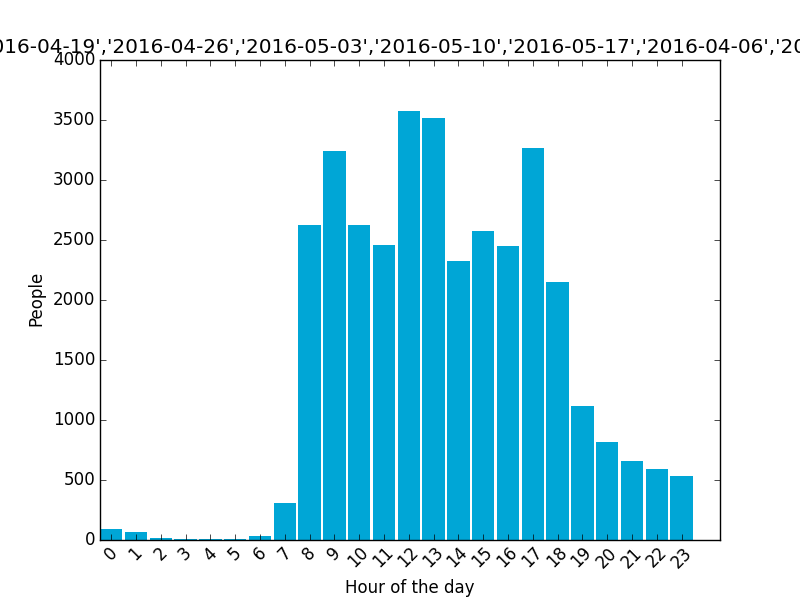
\includegraphics[scale=0.45]{12_weekdays}
	\caption{Movements on weekdays}
	\label{figure:weekdays}
	\end{subfigure}
	\begin{subfigure}[t]{0.48\textwidth}
	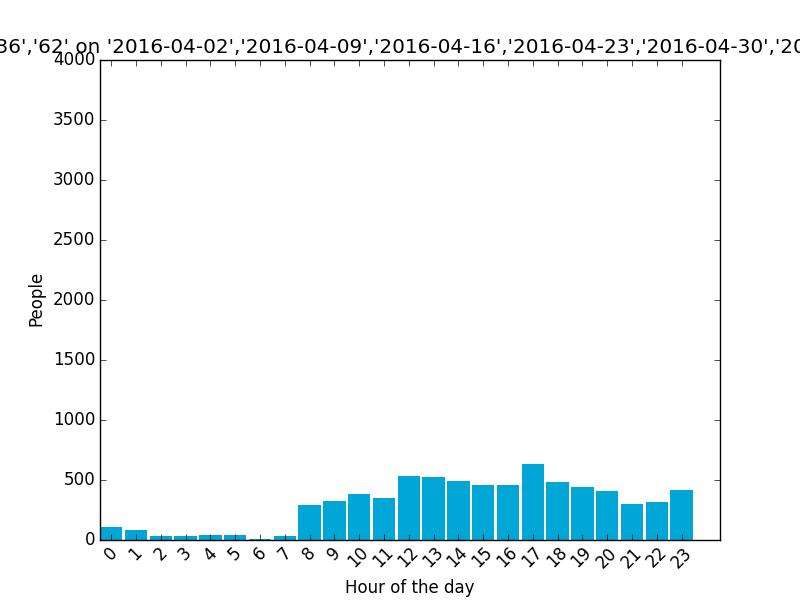
\includegraphics[scale=0.45]{12_weekends}
	\caption{Movement on weekends}
	\label{figure:weekends}
	\end{subfigure}
	\captionsetup{justification=centering}
	\caption{Bar charts of the movements}
\end{figure}

The figures above show the movement from and to the 12 most used buildings on campus. \autoref{figure:weekdays} shows the barplot for the weekdays, \autoref{figure:weekends} shows the barplot for the weekends. It is clear to see that during weekends, there is a lot less movement during weekends. Especially during lunchtime, we can see a peak during weekdays and in the morning and afternoon. In the weekend the movement to the faculties is apparently much less and more spread out over the day.\\
Interesting to see is the movement in the early morning, between 00:00 and 4:00. The library is only open from 8:00 to 2:00, but the bar chart alone does not provide enough information to draw conclusions about these movements.\\\\
\begin{figure}[H]
	\captionsetup[subfigure]{justification=centering}
	\begin{subfigure}[t]{0.48\textwidth}
	\includegraphics[scale=0.4]{12_weekdays_map}
	\caption{Movements on weekdays}
	\label{figure:map_weekdays}
	\end{subfigure}
	\begin{subfigure}[t]{0.48\textwidth}
	\includegraphics[scale=0.65]{12_weekends_map}
	\caption{Movements on weekends}
	\label{figure:map_weekends}
	\end{subfigure}
	\captionsetup{justification=centering}
	\caption{Maps of the movements}
\end{figure}
\autoref{figure:map_weekdays} and \autoref{figure:map_weekends} show the spread of the movement over the whole campus. Now it becomes clear that movement during weekdays is spread out over all faculties, but during weekends is only focused on the Library. There is however one exception, the faculty of 3ME. This could be explained by staff using the building with their campus card. \\

It is interesting to see that during weekdays the movement from and to a faculty is almost always symmetric, whereas in weekends this is certainly not the case. 

\subsection{Architecture as an island}\\
The department of FMRE also assume that architecture students and staff have the tendency to stay in their faculty and move less to other buildings on campus than other faculties. \\
Their question can be answered when looking at the movement between the faculty of architecture and all other buildings. This shows the amount of movement to other faculties, but these amounts need to be compared to the movement from other faculties (for this question IO, CiTG and LR are considered) to other buildings. \\

\begin{figure}[H]
\centering
\includegraphics[scale=0.65]{bk_movement_map}
\captionsetup{justification=centering}
\caption{Movement from the faculty of Architecture}
\label{bk_map}
\end{figure} 

\autoref{bk_map} shows the movement between the faculty of architecture and other faculties. The map shows the 7 most used buildings, the movement to other faculties is only 2\% of the total movement and is left out for readability. The total amount of movement from Architecture is 4.239 people. The largest movement to any other faculty is to the Library with 1.043 people. \\

\begin{figure}[H]
\centering
\includegraphics[scale=0.45]{IO_movement_map.png}
\captionsetup{justification=centering}
\caption{Movement from the faculty of Industrial Design}
\label{io_map}
\end{figure} 

\autoref{io_map} shows the movement from the faculty of Industrial Design to other faculties. The total amount of movement from IO is 10.933 people and the biggest movement is to the faculty of 3ME, with 4.927 people. This is already a lot more movement than the faculty of architecture.\\

\begin{figure}[H]
\centering
\includegraphics[scale=0.65]{citg_movement_map.png}
\captionsetup{justification=centering}
\caption{Movement from the faculty of Civil Engineering}
\label{citg_map}
\end{figure} 

\autoref{citg_map} shows the movement from the faculty of Civil Engineering to other faculties. The total amount of movement from CiTG is 11.035 people and the biggest movement is to the faculty of EWI, with 2.897 people. This is even more movement than IO.\\

\begin{figure}[H]
\centering
\includegraphics[scale=0.65]{lr_movement_map.png}
\captionsetup{justification=centering}
\caption{Movement from the faculty of Aerospace Engineering}
\label{lr_map}
\end{figure} 

\autoref{lr_map} shows the movement from the faculty of Aerospace Engineering to other faculties. The total amount of movement from AE is 4.348 people and the biggest movement is to the Fellowship, with 2.435 people. \\
Looking at these figures we can clearly see that the movement from the faculty of architecture is much less than the movement from Civil Engineering and Industrial Design.  However, the faculty of Aerospace Engineering seems to be even more isolated than architecture. 


%%\chapter{Context}\label{context}
\section{Use case: TU Delft}
% Matthijs
% Information about location
This projects main area of interest is the campus of the TU Delft. There are more than 30.000 users using the campus on more than 150 hectares. This emphasises even more the magnitude of this project. The eduroam network logs the devices connected to the access points, which implicitly means logging the (approximate) location of the person carrying the device and more information. This tracking data can be used to derive information about the personality of the person carrying the device, such as the distinction between staff and students, based on the tracked locations. Connection to the Wi-Fi eduroam network is free of charge and requires only a NetID, which all students and staff get upon registration at the university. \\\\
It is very important to understand, that 'no data is also data'. This means that a devices that is not being tracked by any access point for a period of time, is either off-campus or disconnected and still on campus. This provides valuable information when researching the movement patterns. This will be further discussed in the \autoref{preprocessing}. \\\\
The eduroam network of the TU Delft campus consists of 1730 access points, distributed over more than 30 buildings. The data is collected for each of the access points over a period of little more than 3 months. The logs are stored in a database on a virtual server, where it is accessible to the three project groups and the Geomatics staff. The data that is collected and the storage in the database is further described in \autoref{datadescriptionandsystemofaps}. \\\\
The department of Facility Management and Real Estate (FMRE) is the main client for the entire Synthesis Project. They would like to know how the campus is being used, what the hotspots on campus and in buildings are, when people travel the most from one building to another and which buildings are most visited.

\section{Previous research: Rhythm of the campus}
% Matthijs
% Summary of their summary
In the fall of 2014, similar research was conducted during another edition of the Geomatics Synthesis Project. The group "Rhythm of the campus" investigated the use of the Library and the Aula of the TU Delft, to gain insight in patterns the use of the facilities of the Library and Aula. This section will give a short summary of their research (\cite{rhythmofthecampus}).\\\\
During the project, the group used passive Wi-Fi monitoring to detect users of the TU Delft Library and the Aula to gain insight in the occupation, in request of FMRE. They used BlueMark sensors at the Library, Aula and 5 other faculties for a period of one week and collected ground truth data for 2 days. Due to its sheer size, the raw data was difficult to process. The data was filtered from static devices and outliers and the data analysis resulted in identification of the occupation of the Library and the Aula. The end results was a dashboard which visualized the sensor network, data analysis and pattern recognition to help the client in the decision making process.\\\\
This research was different from the research conducted in this Synthesis Project, mainly due the larger size of the eduroam network and the ability to track everybody using the Wi-Fi network.

\section{Privacy}
This project focuses on identifying common movement patterns, ignoring the individual, therefore we did not test explicitly whether is possible to identify individuals or not from the data. However, based on our findings about the operation of the eduroam Wi-Fi network and about the methods that
are used to identify movement patterns, we can make the following assumptions.\\\\
Movement patterns are rather unique, therefore it is possible to match them to individuals even if maybe not in every case. However, in order to do so it is
necessary to have additional data available. This additional data itself is often considered private data, e.g. the complete weekly schedule of the person.
Provided that timetables are openly accessible and the occupation of the individual is known, then his movement pattern may be identified in the dataset.\\\\
The availability of a detailed access point map makes it easier to identify individuals by allowing a more detailed movement analysis (e.g. on building-part
level). It reduces the ambiguity that is still present in building level movement analysis.

\section{Data validation}
The spatial accuracy of the Wi-Fi log dataset is defined by the range of the APs. Although we do not have information on the exact range of the different
APs, we estimate the range to be a few tens of meters. Therefore, if a user is recorded by a specific AP, in reality he can be anywhere around the AP in its
range.\\\\
The temporal accuracy of the Wi-Fi log dataset is defined by the five minute campus-wide logging interval of the eduroam system. It means that all APs on the TU Delft campus log all connected devices at the same moment in approximately five minute intervals. Therefore, it is possible that the user is already at a given AP, but he will be first recorded at the next scan round, or the user already left the AP but that also will be only recorded at the next scan round.

\section{Representativeness}
% Xander
In the GSP a big amount of Wi-Fi logging data is used. The data represents all people that make (active) use of the eduroam network. These are the students and employees of the TU Delft.  There is just a small amount of people that are within the spatial scope of the project and cannot connect to eduroam. The data is acquired by the access points, which all are located in a building on the campus. The people that use a building on the campus, but do not make use of the eduroam network, is a very small part. Thus, the main part of actual users is covered by the data used in the GSP. The collection of data is acquired over a continuous time interval of more than 2 months. This time period would be large enough to reflect on all users of the campus to some extend.
\section{Data description and System of APs}\label{datadescriptionandsystemofaps}
\subsection{Data description}\label{datadescription}
This section will describe the main data source used within the Geomatics Synthesis Project; a PostgreSQL database containing the logs from the Wi-Fi access points on the TU Delft campus. The wifilog table has several column, with a data value for each row (\autoref{segmentwifilog}).\\\\
\begin{table}[H]
	\centering
	\captionsetup{justification=centering}
	\caption{A segment of the main data source; the wifilog table}
	\label{segmentwifilog}
	\begin{tabular}{@{}lllllllll@{}}
		\toprule
		\textbf{username} & \textbf{mac} & \textbf{asstime} & \textbf{apname}  & \textbf{maploc}                                                     & \textbf{sesdur} & \textbf{snr} & \textbf{rssi}          \\ \midrule
		j85cCQ..      & l6iOu+.. & 14-4-2016 12:30  & A-23-0-029 & ..CITG \textgreater 4e Verdieping       & 1:32:02         & 35           & -57\\
		wrBqM..       & f2Pw/P.. & 14-4-2016 7:49   & A-23-0-035 & ..CITG \textgreater 5e \& 6e Verdieping & 5:32:16         & 37           & -56\\
		wrBqM..       & f2Pw/P.. & 14-4-2016 13:22  & A-23-0-035 & ..CITG \textgreater 5e \& 6e Verdieping & 0:40:20         & 46           & -50\\
		wrBqM..       & f2Pw/P.. & 14-4-2016 14:02  & A-23-0-093 & ..CITG \textgreater 5e \& 6e Verdieping & 1:27:13         & 11           & -86\\
		wrBqM..       & f2Pw/P.. & 14-4-2016 15:29  & A-23-0-091 & ..CITG \textgreater 5e \& 6e Verdieping & 0:05:08         & 30           & -65\\
		wrBqM..       & f2Pw/P.. & 14-4-2016 15:34  & A-23-0-035 & ..CITG \textgreater 5e \& 6e Verdieping & 1:42:32         & 29           & -65\\
		J0IwA+..      & HkLY1U.. & 14-4-2016 11:33  & A-23-0-035 & ..CITG \textgreater 5e \& 6e Verdieping & 1:27:40         & 33           & -59\\
		J0IwA+..      & HkLY1U.. & 14-4-2016 13:01  & A-23-0-035 & ..CITG \textgreater 5e \& 6e Verdieping & 1:01:01         & 26           & -68\\
		J0IwA+..      & HkLY1U.. & 14-4-2016 14:02  & A-23-0-035 & ..CITG \textgreater 5e \& 6e Verdieping & 3:30:19         & 25           & -68\\
		J0IwA+..      & HkLY1U.. & 14-4-2016 17:32  & A-23-0-035 & ..CITG \textgreater 5e \& 6e Verdieping & 0:40:05         & 27           & -69\\ \bottomrule
	\end{tabular}
\end{table}
The data value for each attribute (column) in the wifilog table will be described in more detail.\\\\
\textbf{Username}\\
The username column provides the username, as a hashed text. Every user has a unique username, but can appear in the data more than once.
\\\\
\textbf{Mac}\\
The mac column provides the media access control adress (MAC address), as a hashed text. The MAC address is a unique identifier assigned to a specific piece of hardware, such as the network adapter located in Wi-Fi devices (mobile phones, tablets, laptops etc.). So, it would be possible that a user can have more than one device connected to the Wi-Fi eduroam network at the same time.
\\\\
\textbf{Asstime}\\
The asstime is the time of which a connected device is recorded by the system.
\\\\
\textbf{Apname}\\
The apname is the name assigned to the access point. Every access point has a unique name. 
\\\\
\textbf{Maploc}\\
The maploc describes the location of the access point. There could be multiple access points with the same maploc. For instance, there are 31 access points located on the ground floor of the Faculty of Architecture and the built environment.\\
\begin{figure}[H]
	\centering
	\includegraphics[scale=0.15]{sesdur_graph_without5min.png}
	\captionsetup{justification=centering}
	\caption{The frequency of session durations}
	\label{frequency_sesdur}
\end{figure}
\textbf{Sesdur}\\
The sesdur describes the session duration of which a device is connected to the access point. Because this is not as straightforward as it seems, this will be explained more extensively. \autoref{frequency_sesdur} shows the frequency of session durations (the peak at exactly 5 minutes is filtered out to make the graph more readable). There is a large peak at exactly 5 minutes, a peak at approximately 5 minutes and decreasing peaks after a time interval of approximately 5 minutes. It looks like it is recording in a certain time interval in which the device is (still) connected. \\\\
In order to justify this, the query below is used to see the asstimes (and time to next asstime)\\\\
\begin{center}
\begin{lstlisting}[language=SQL]
select *, asstime_next-asstime as difference
from (
	select count(*),asstime, lead(asstime) over (order by asstime) asstime_next
	from wifilog
	where extract(day from asstime) = 4
	and extract(month from asstime) = 4
	and extract(year from asstime) = 2016
	group by asstime
	order by asstime) as subquery
\end{lstlisting}
\end{center}
\begin{table}[H]
	\centering
	\captionsetup{justification=centering}
	\caption{The time and time to next scan at a random day}
	\label{timetonextscan}
	\begin{tabular}{@{}llll@{}}
		\toprule
		count & asstime        & asstime\_next  & difference \\ \midrule
		2578  & 4-4-2016 13:04 & 4-4-2016 13:09 & 0:05:10    \\
		2435  & 4-4-2016 13:09 & 4-4-2016 13:15 & 0:05:11    \\
		2486  & 4-4-2016 13:15 & 4-4-2016 13:20 & 0:05:11    \\
		2530  & 4-4-2016 13:20 & 4-4-2016 13:25 & 0:05:11    \\
		2471  & 4-4-2016 13:25 & 4-4-2016 13:30 & 0:05:11    \\
		2444  & 4-4-2016 13:30 & 4-4-2016 13:35 & 0:05:11    \\
		2524  & 4-4-2016 13:35 & 4-4-2016 13:40 & 0:05:11    \\
		2588  & 4-4-2016 13:40 & 4-4-2016 13:46 & 0:05:12    \\
		2690  & 4-4-2016 13:46 & 4-4-2016 13:51 & 0:05:11    \\
		2560  & 4-4-2016 13:51 & 4-4-2016 13:56 & 0:05:11    \\ \bottomrule
	\end{tabular}
\end{table}
\autoref{timetonextscan} shows that the time to the next scan is 5 minutes and several seconds in all cases. Most important to know is that all access points are logging the connected device(s) at the same time campus wide. \\\\                                                       
\autoref{sesdur_example} will be used to explain the way the time interval of approximately 5 minutes is coming back in the session duration.\\\\
The first record shows the device is not connected to any of the access points on the campus in the subsequent moment of recording, resulting in a session duration of exactly 5 minutes. The last record in \autoref{sesdur_example} shows the result of a device that is still connected to the same access point at the subsequent moment of recording. In this case the session duration will be 10 minutes and 21 seconds. This is the time interval between the first moment the device is recorded and the first time the device is not recorded by the same access point anymore. The record with id number 6 describes a situation in which the device is connected to an access point at the moment of recording and connected to another access point at the subsequent moment of recording, the session duration is 5 minutes and 18 seconds in this case. This is the time interval between the two moments of recording. This time interval can vary, but is always approximately 5 minutes.\\\\
\begin{table}[H]
	\centering
	\captionsetup{justification=centering}
	\caption{Varying session durations}
	\label{sesdur_example}
	\begin{tabular}{@{}lllllll@{}}
		\toprule
		\textbf{id} & \textbf{username} & \textbf{mac} & \textbf{asstime} & \textbf{apname} & \textbf{maploc}                                                                     & \textbf{sesdur} \\ \midrule
		1           & oHh0Sz..      & WWW0Cd.. & 1-4-2016 10:13   & A-12-0-104      & ..\& Proeffabriek \textgreater !e Verdieping                 & 0:05:00         \\
		2           & oHh0Sz..      & WWW0Cd.. & 1-4-2016 10:18   & A-132-0-064     & ..32-OCP-IO \textgreater 1e Verdieping                     & 0:20:27         \\
		3           & oHh0Sz..      & WWW0Cd.. & 1-4-2016 11:36   & A-132-0-105     & Root Area                                                                           & 0:15:22         \\
		4           & oHh0Sz..      & WWW0Cd.. & 1-4-2016 11:51   & A-132-0-066     & ..32-OCP-IO \textgreater 1e Verdieping                     & 0:20:35         \\
		5           & oHh0Sz..      & WWW0Cd.. & 1-4-2016 14:01   & A-132-0-069     & ..32-OCP-IO \textgreater 1e Verdieping                     & 0:05:43         \\
		6           & oHh0Sz..      & WWW0Cd.. & 1-4-2016 14:06   & A-132-0-133     & ..32-OCP-IO \textgreater 4e Verdieping                     & 0:05:18         \\
		7           & oHh0Sz..      & WWW0Cd.. & 1-4-2016 14:12   & A-132-0-066     & ..32-OCP-IO \textgreater 1e Verdieping                     & 0:05:10         \\
		8           & oHh0Sz..      & WWW0Cd.. & 1-4-2016 14:17   & A-132-0-104     & ..32-OCP-IO \textgreater 2e Verdieping                     & 0:05:10         \\
		9           & oHh0Sz..      & WWW0Cd.. & 1-4-2016 14:22   & A-132-0-067     & ..32-OCP-IO \textgreater 1e Verdieping                     & 0:05:10         \\
		10          & oHh0Sz..      & WWW0Cd.. & 1-4-2016 14:27   & A-132-0-066     & ..32-OCP-IO \textgreater 1e Verdieping                     & 0:10:21         \\ \bottomrule
	\end{tabular}
\end{table}
\textbf{SNR}\\
The signal to noise ratio(SNR) describes a measurement that compares the signal strength to the level of background noise (in dB).\\\\
\textbf{RSSI} \\
The received signal strength indicator (RSSI) describes the received signal strength (in dB).

\subsection{System of APs}\label{systemofaps}
This section will describe the current layout of access points (APs) on the TU Delft campus. The location of APs in a building is not known, but for the Faculty of Architecture and the built environment a paper map was available. Therefore the system of APs in the Faculty of Architecture and the built environment will be described in more detail. \\\\
In total there are 1730 access points, distributed over more than 30 buildings on the campus. The access points are mostly placed on walls or ceilings. The data describes that every access point is linked to a certain location. Due to the (wide) signal range of the access point, the device can be located at a different floor level than the access point it is connected to. Moreover, there could be access points located at the first floor while serving people at ground floor as well. This is the case in rooms with high ceilings, such as the orange hall in the Faculty of Architecture and the built environment. \\\\
As said, the Faculty of Architecture and the built environment is the only building of which the location of the access points are known. The floor plans are enriched with the location of the access point (see \autoref{apmap_west}). Next to that, a table is provided with additional information regarding the access points, although this table does not contain all present access points. This table includes the MAC address of the access point. This could be used to look up to what access point the device is connected.\\\\
\begin{figure}[H]
	\centering
	\includegraphics[scale=0.6]{apmap_west.png}
	\captionsetup{justification=centering}
	\caption{Ground floor plan with the location of the access points}
	\label{apmap_west}
\end{figure}


%% Use letters for the chapter numbers of the appendices.
\appendix

%\input{appendix-a}

%\bibliography{report}

\end{document}

